\chapter{Ergebnisse der Lokalisierung}
\section{Methodik}
\begin{figure}{!ht}
	\centering
	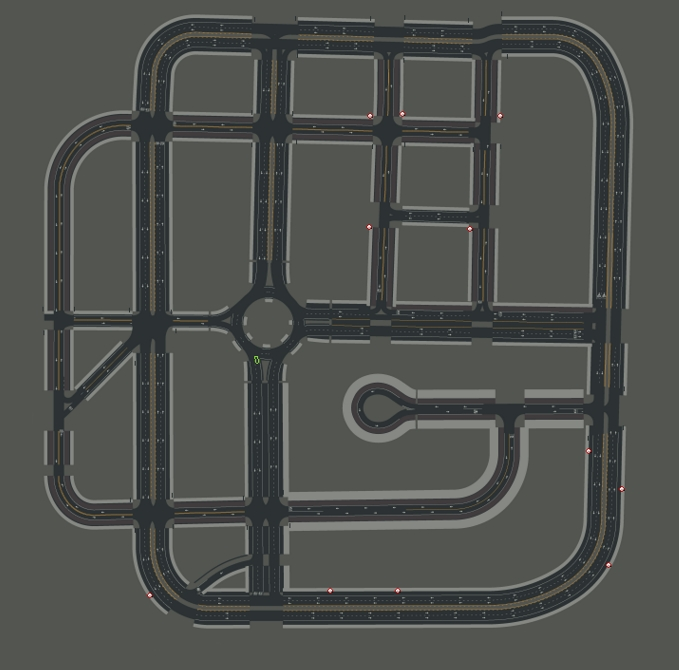
\includegraphics[width=0.45\textwidth]{07_Town03.jpg}
	\caption[CARLA Simulator Karte Town03]{CARLA Simulator Karte Town03. (CARLA Dokumentation, 2022)}
\end{figure}

Für die Datenerhebung wurde im CARLA Simulator die Umgebung 'Town03' ausgewählt. Die CARLA Dokumentation beschreibt Town03 als abwechslungsreichste und komplexeste Karte des Simulators. Town03 beinhaltet eine gro{\ss}e Kreuzung, Erhebungen, Kreisverkehr und einen Tunnel.
\newline

Es wurden Daten für 5 unterschiedliche Witterungsverhältnisse erhoben: sunset, clear night, default, hard rain, wet sunrise. Die Witterungsverhältnisse wurden über CARLAs Python API gesetzt.
\newline 

Für jedes Witterungsverhältnis wurden 5 Testfahrten aufgezeichnet. Die Testfahrten sind zufällige Strecken. Au{\ss}erdem wurden für alle Fahrten 50 NPCs auf der Karte gespawnt. NPC beinhalten andere Fahrzeuge sowie Fu{\ss}gänger. Die Geschwindigkeit des Testfahrzeugs variiert zwischen 30 und 100 $\frac{km}{h}$, je nach Streckenabschnitt.
\newline

Bei jeder Testfahrt waren die Stereokamera und die RGB-D Kamera am Fahrzeug angebracht, das Bild der linken RGB Kamera wurde in beiden verwendet. Die ROS Nodes für beide Visuellen Odometrie Programme laufen bei allen Fahrten live mit und alle Ausgangsdaten wurden über das ROS Werkzeug rosbag in eine sql3 Datenbank geschrieben.
\newline

Ein Verarbeitunsgtool 'BagParser' wurde geschrieben um Daten aus den rosbag Datenbanken zu extrahieren und in .txt Dateien, OpenCV Matritzen oder Quarternion formatierte .txt Dateien abzulegen. 
\newline

Die Bewertung von geschätzten Trajektorien bringt einige Herausforderungen mit sich. 

Zum einen referenzieren Ground Truth und die Schätzung unterschiedliche Koordinatensysteme. Ground Truth referenziert das Fahrzeugkoordinatensystem währen die VO Schätzung das Koordinatensystem der linken Kamera referenziert. Die Positionen müssen also zuerst aneinander angeglichen werden, bevor ein Vergleich durchgeführt werden kann. 
\newline

Ein anderes Problem ist die Fehlerfortpflanzung. Es kann sein, dass an einer Stelle ein Winkel mit gro{\ss}er Abweichung zu Ground Truth geschätzt wurde. Folgende Schätzungen sind vielleicht mit wesentlich kleineren Fehlern behaftet, zeigen im absoluten Vergleich aber noch den vorherigen Fehler. 

Es handelt sich bei den Daten au{\ss}erdem um hochdimensionale Datensätze; die Anzahl der Merkmale ist höher als die Anzahl der Beobachtungen.
\newline

Um mit diesen Herausforderungen umzugehen wurden die Daten basierend auf dem Paper \textit{Rethinking Trajectory Evaluation for SLAM: a Probabilistic, Continuous-Time Approach}\cite{zhangSLAM} und der Trajectory Evaluation Toolbox aus \textit{A Tutorial on Quantitative Trajectory Evaluation for Visual(-Inertial) Odometry} \cite{errorEst} bewertet.
\newline

Voraussetzung für eine Evaluation ist zuerst die gleiche Ausrichtung der geschätzten Trajektorien mit Ground Truth. Die beiden sind durch eine euklidische Transformation im 3 Dimensionalen Raum miteinander verbunden. Die Transformationen bestehen aus Rotation und Translation und werden Formal als Spezielle Euklidische Transformation SE(3) bezeichnet. Anstatt mit Rotationsmatritzen zu rechnen werden für die Auswertung mit rotations Quaternionen gerechnet. Quaternionen sind ein eigener Zahlenbereich und eine Erweiterung des Zahlenbereichs der reellen Zahlen. Als Vorbereitung der Auswertung müssen die Trajektorien daher als Messreihe von 7-Dimensionalen Vektoren abgelegt werden 
\begin{equation}
	\centering
		X_i = (x\; y\; z\; q_w\; q_x\; q_y\; q_z)^\top 
\end{equation}

Die Ausrichtung wird durch eine Methode der Kleinsten Quadrate Implementation für zwei Punktmengen nach Umeyama \cite{Umeyama1991LeastSquaresEO} gelöst.

\begin{equation}
	\centering
	\underset{R,T,s}{\arg\min} \sum_{i = 0}^{N} \| \hat{t}_i -sR_{ti} -T \|^2   
\end{equation}

Mit Ground Truth Posen als $\hat{t}$ und Schätzung durch Visuelle Odometrie als $s$. 
\newline

In der Auswertung werden für jede Strecke der absolute Streckenfehler ATE (Absolute Trajectory Error) und der relative Fehler (RE) berechnet. Ground Truth sei $X_{gt}$ und die, bereits ausgerichtete, geschätzt Trajektorie sei $\hat{X}'$. Die Trajektorie ist der zeitlicher Verlauf der Zustände der VO Schätzung. Für einen einzelnen Zustand wird der Fehler zwischen $\hat{x}'_i$ und Ground Truth $x_i$ definiert als  
\begin{equation}
	\Delta x_i = \{\Delta R_i, \Delta p_i\}
\end{equation}
für die gilt
\begin{equation*}
	R_i = \Delta R_i \hat{R}'_i,\:
	p_i = \Delta R_i \hat{p}'_i	
\end{equation*}

mit der Rotationsmatrix $R$ und der Position $p$. Dadurch errechnet sich der absolute Fehler zu 

\begin{align}
	\Delta R_i &= R_i (\hat{R}'_i)^\top,\\
	\Delta p_i &= p_i - \Delta R_i \hat{p}'_i
	\label{eq:absoluteErr}
\end{align}

Nun kann, um den die Qualität der Gesamtstrecke zu quantifizieren, die Quadratwurzel des mittleren quadratischen Fehlers (root mean square error (RMSE)) gebildet werden
\begin{align}
	ATE_{rot} &= (\frac{1}{N} \sum_{i = 0}^{N-1} \|\angle (\Delta R_i)  \|^2 )^\frac{1}{2},\\
	ATE_{pos} &= (\frac{1}{N} \sum_{i = 0}^{N-1} \| (\Delta p_i)  \|^2 )^\frac{1}{2}
\end{align}

wobei $\angle(\cdot)$ für die Konvertierung der Schreibweise von Matrixform zu Euler-Winkel.
\newline
\newline

Zusätzlich wird der relative Fehler berechnet. Der von Zhang et al. \cite{errorEst} vorgeschlagene Ansatz ist, die relative Beziehung zwischen den Zuständen zu verschiedenen Zeiten zu messen. Das gemeinsame Kriterium der Zustände ist die zurückgelegte Distanz. Es wird also die Gesamtstrecke und die Schätzung der Gesamten Stecke in Teilstrecken $s$ und $e$ für den Abschnitt $\mathfrak{F}$ zerlegt. 
\newline

Für jeden Teilabschnitt werden aus den Messwerten Gruppen mit $K$ Zustandspaaren zusammengefasst. Die Menge der Paare $d_k$ bilden jeweils eine Trajektorie für den Streckenabschnitt $\mathfrak{F}$. 

\begin{equation}
	\mathfrak{F} = \{d_k\}^{K-1}_{k=0}, \:\:\: d_k= \{ \hat{x}_s, \hat{x}_e
\end{equation}

Der relative Fehler $\delta d_k$ berechnet sich auf die gleiche Weise wie der absolute Fehler \ref{eq:absoluteErr}. Somit ergibt sich der Fehler $\delta d_k$  für ein Wertepaar $d_k$ aus

\begin{align}
	\delta \phi_k & = \angle \delta R_k = \angle R_e(\hat{R'_e})^\top,\\
	\delta p_k &= ||p_e - \delta R_k \hat{p}'_e||^2.
\end{align}

Daraus ergibt sich eine Menge von Werten, jeweils einer pro Teilabschnitt. Die Menge wird formal beschrieben durch 

\begin{align}
	RE_{rot} \: &= \: \{\delta \phi_k\}^{K-1}_{k=0},\\
	RE_{pos} \: &= \: \{\delta p_k\}^{K-1}_{k=0},\\
\end{align}

Die Abbildung dieser Mengen ist in den Boxplots zu sehen. Der mittlere Kasten besteht aus zwei Quartilen und dem Median. Der Median ist der Strich, die Quartile beinhalten sämtliche Schätzfehler. Die Antennen bzw Whiskers bilden das obere und untere Quartil.

\newpage
\section{Ergebnisse}
%%%%%%%%%%%%%%%%%%%%%%%%%%%
\begin{figure}[!ht]
	\centering
	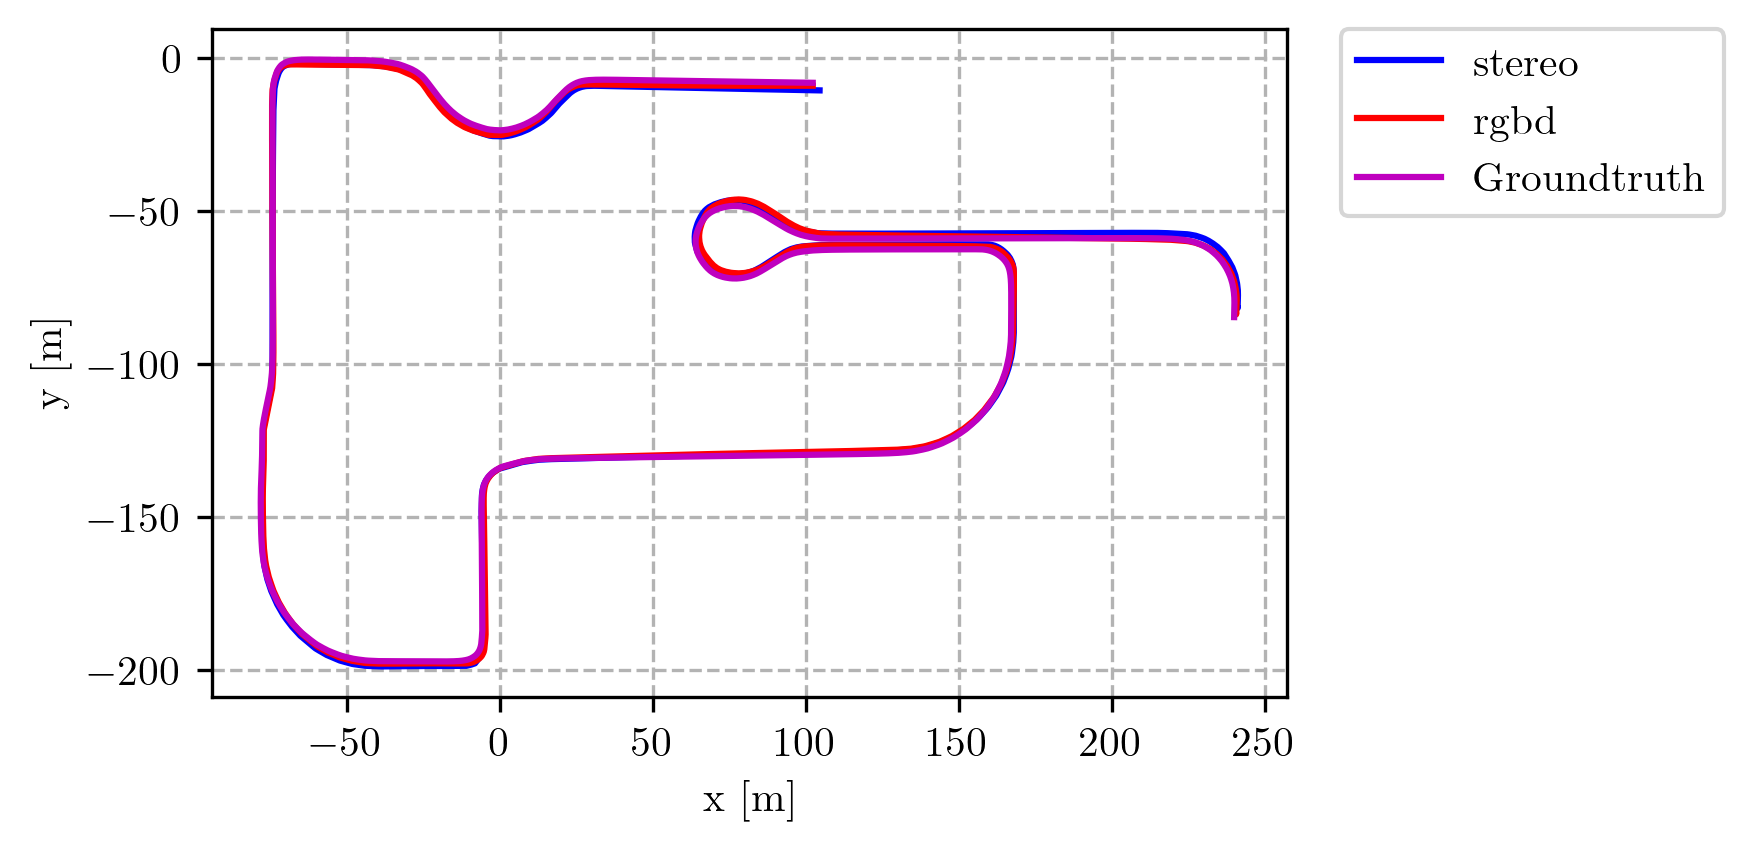
\includegraphics[width=\textwidth]{vorzeigestrecke/default_01_trajectory_top.png}
	\caption[Plot der Trajektorien Teststrecke 'Default 01']{Trajektorien Ground Truth und Schätzung durch Visuelle Odometrie der Teststrecke 'Default 01'}
\end{figure}

Es wurden insgesamt Daten für 25 Testfahrten erhoben. Der Datensatz einer Testfahrt besteht immer aus den Ground Truth Odometrie Daten, der durch RGB-D geschätzten Odometrie und der durch Stereo geschätzten Odometrie. Zugunsten der Übersichtlichkeit werden nicht alle Strecken und Daten grafisch aufbereitet. Stattdessen wurden Daten einzelner Strecken als Stichproben abgebildet um einen intuitiven Einblick in die Ergebnisse zu vermitteln. 

	\begin{figure}[!ht]
	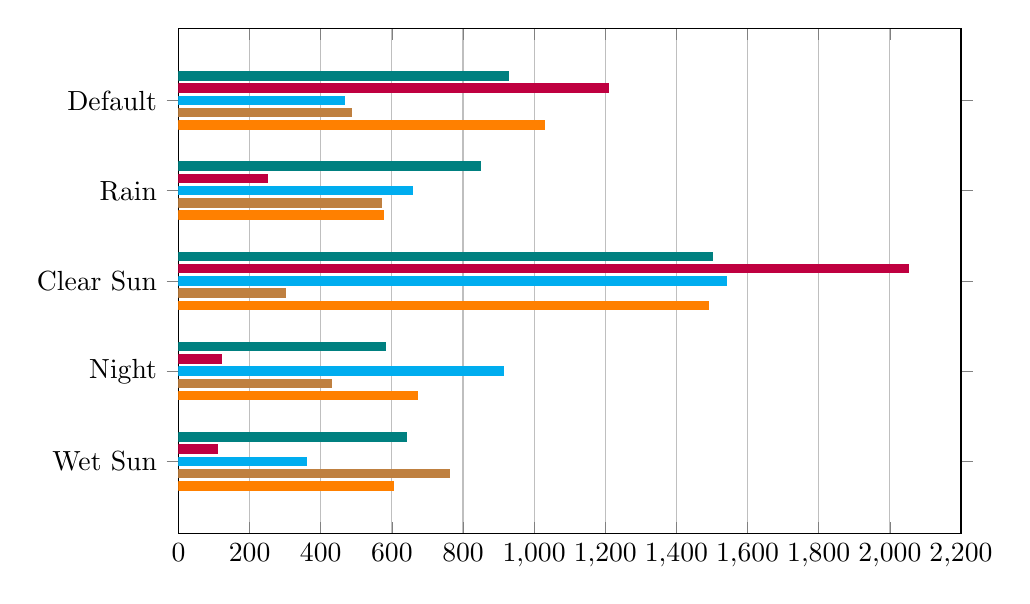
\begin{tikzpicture}
  \begin{axis}
      [
        width  = .95\textwidth,
        height = 8cm,
        xbar = .05cm,
        bar width=3pt,
        xmajorgrids = true,
        xmin = 0, 
        xmax = 2200,
        ytick=data,
        %enlarge x limits = {value = .25, upper},
        enlarge y limits = {abs = .8},
        yticklabels={Wet Sun, Night, Clear Sun, Rain, Default}
      ]
      %Run 1 bei allen
      \addplot[xbar][style={orange,fill=orange,mark=none}]
      coordinates {(604,0) (672,1) (1491,2) (575,3) (1029,4)};
      %Run 2 bei allen
      \addplot[xbar][style={brown,fill=brown,mark=none}]
      coordinates {(763,0) (429,1) (301,2) (571,3) (486,4)};
      %Run 3 bei allen
      \addplot[xbar][style={cyan,fill=cyan,mark=none}]
      coordinates {(359,0) (915,1) (1540,2) (658,3) (466,4)};
      %Run 4 bei allen
      \addplot[xbar][style={purple,fill=purple,mark=none}]
      coordinates {(109,0) (121,1) (2052,2) (249,3) (1208,4)};
      %Run 5 bei allen
      \addplot[xbar][style={teal,fill=teal,mark=none}]
      coordinates {(641,0) (582,1) (1500,2) (850,3) (929,4)};
  \end{axis}
\end{tikzpicture}
	\caption[Testfahrten Streckenlängen]{Streckenlängen aller 25 Testfahrten in m.}
\end{figure}

Die Datensätze Simulieren unterschiedliche Sichtverhältnisse. Es sei angemerkt das die Fahrzeuge im CARLA Simulator über keine eigenen Lichtquellen verfügen.

\begin{figure}[!ht]
	\begin{tabular}{lll}
		1 & 	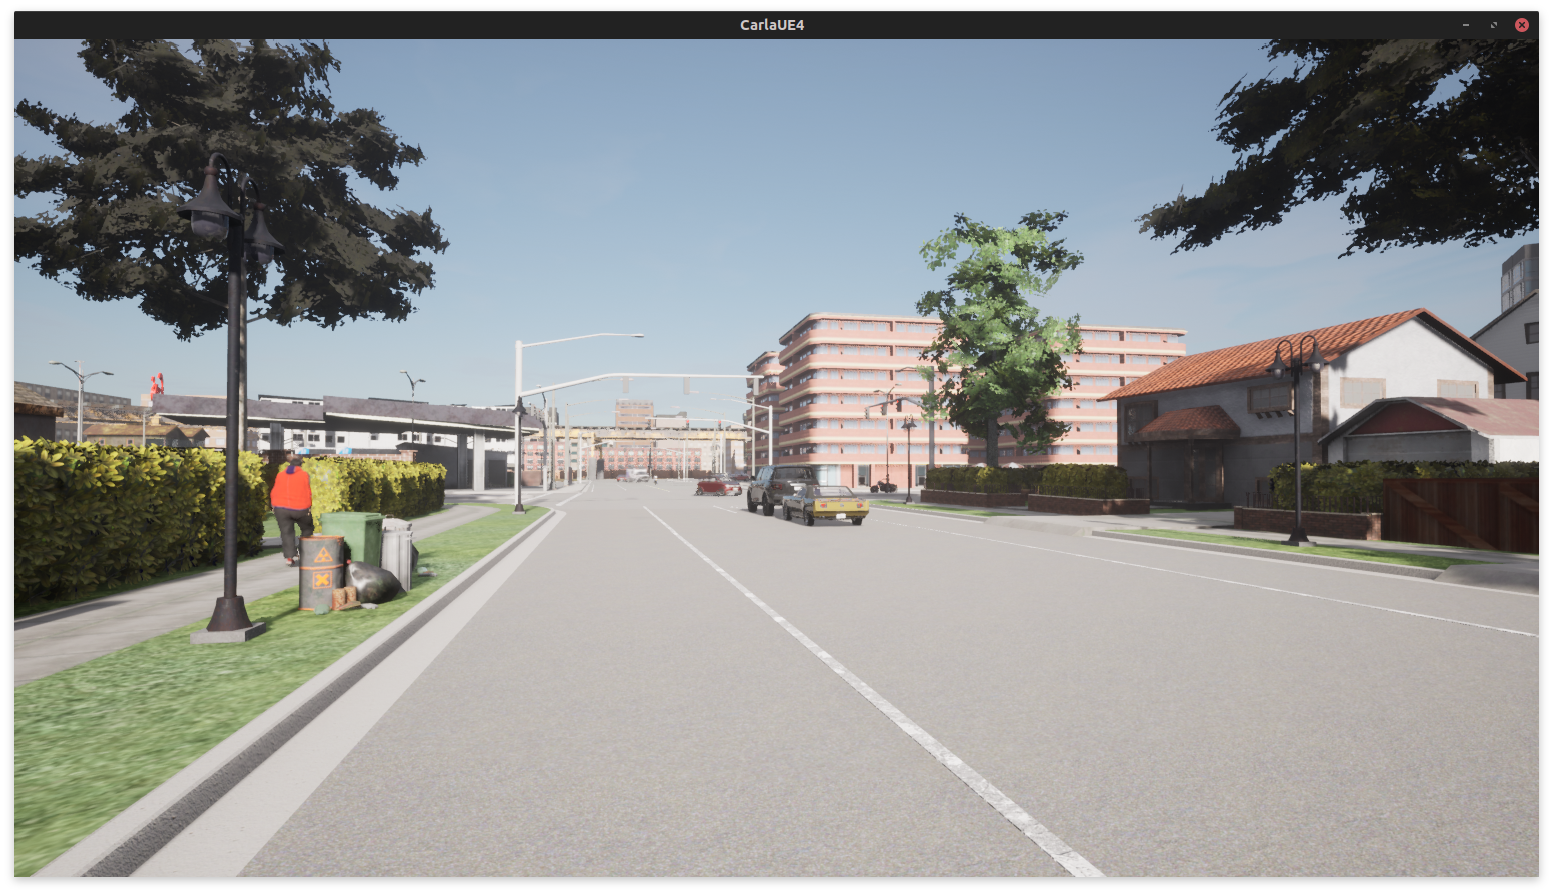
\includegraphics[width=.4\textwidth]{07_default.png} &
		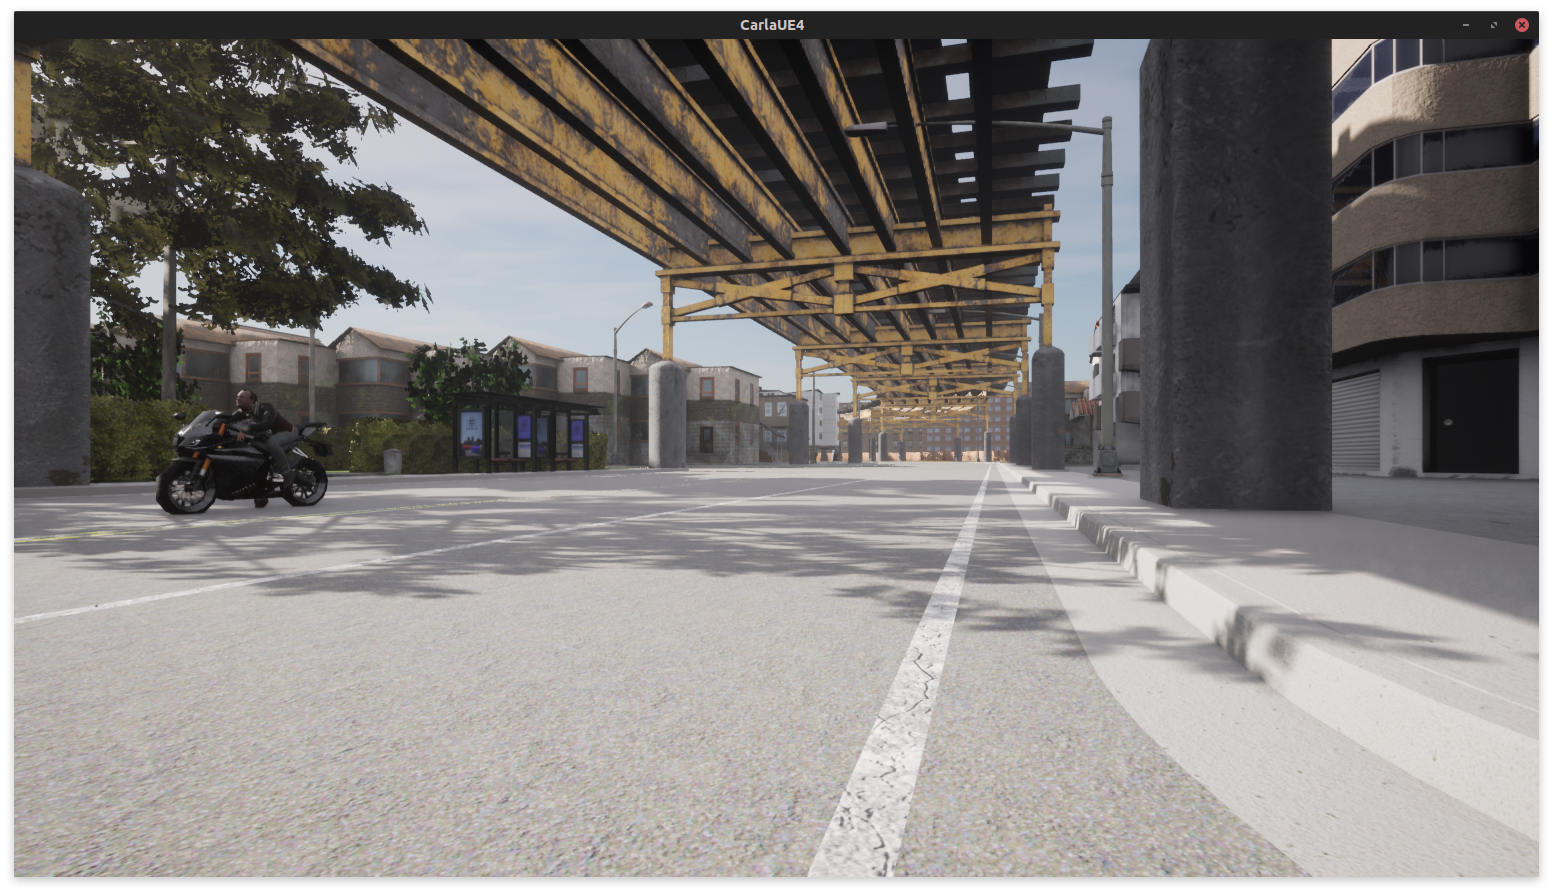
\includegraphics[width=.4\textwidth]{07_default03.png}\\
		2 & 	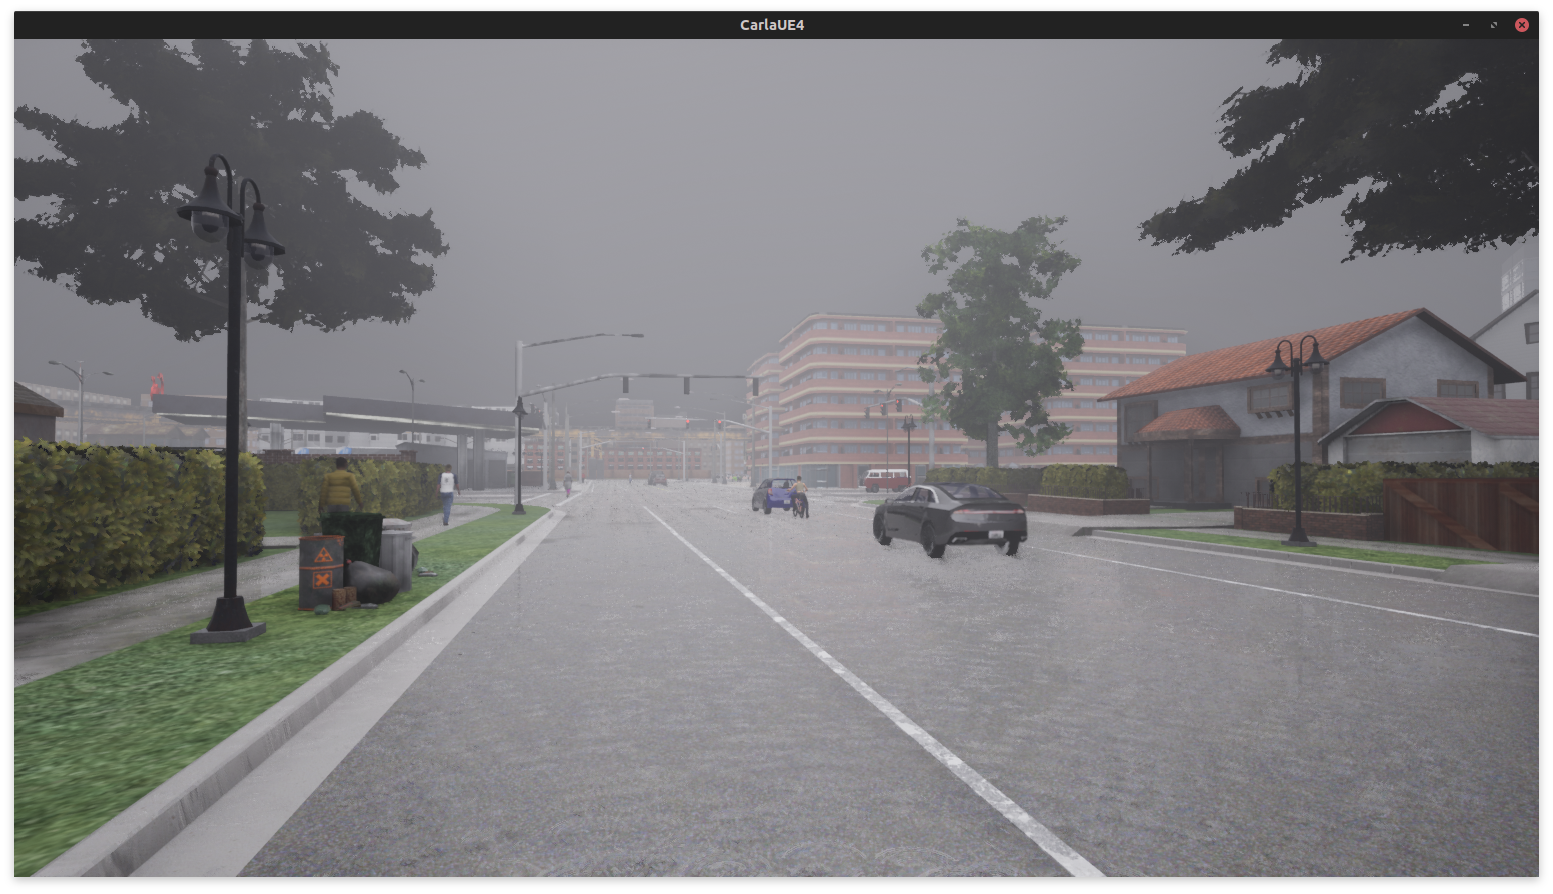
\includegraphics[width=.4\textwidth]{07_hard_rain.png} &
		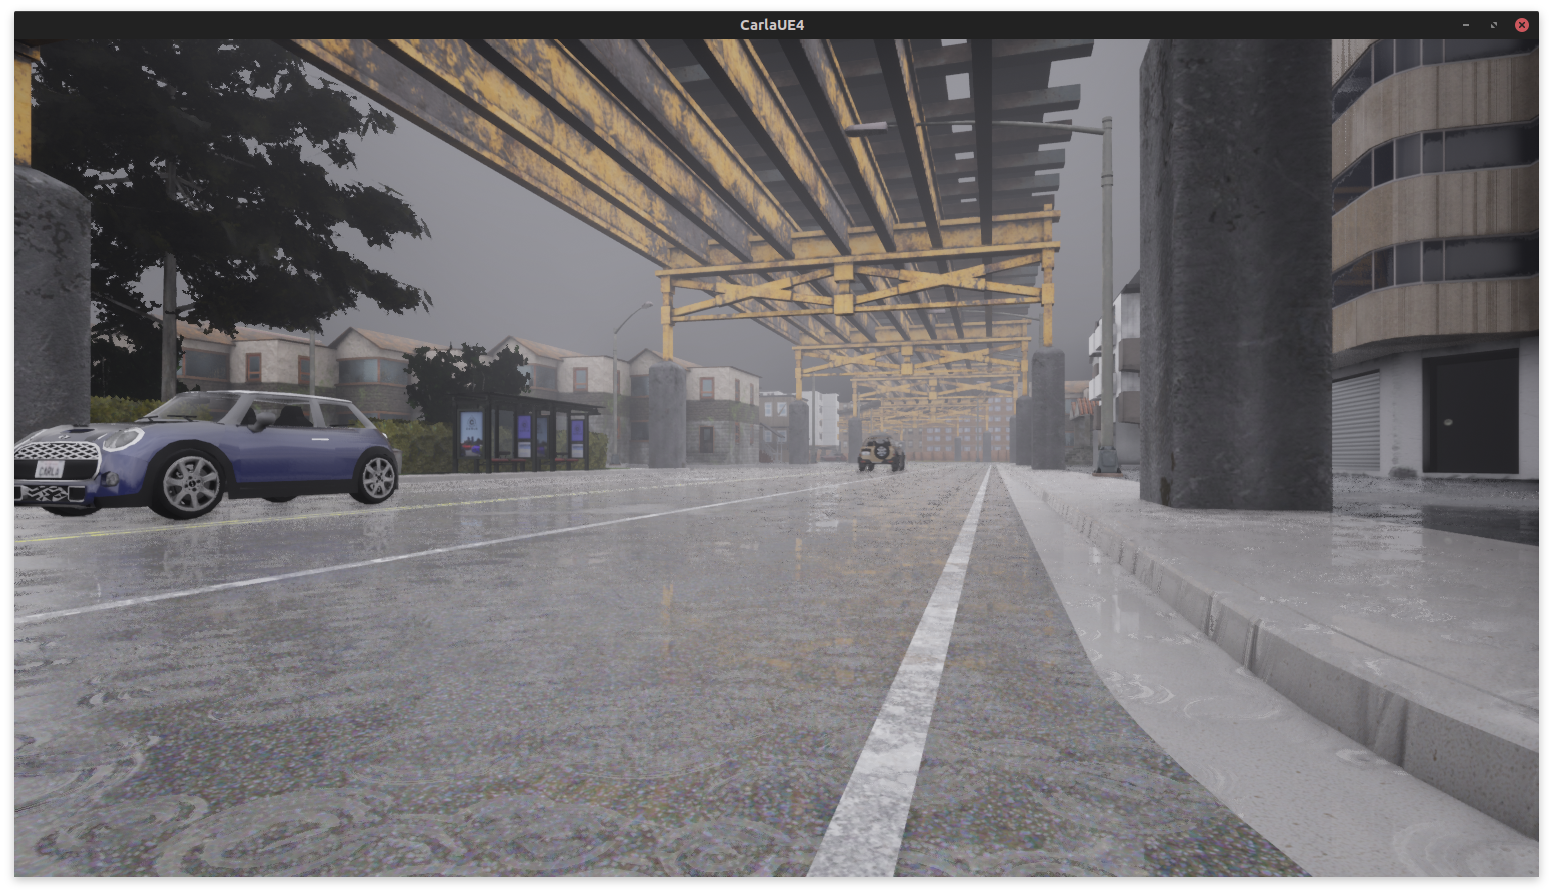
\includegraphics[width=.4\textwidth]{07_rain_noon03.png}\\
		3 & 	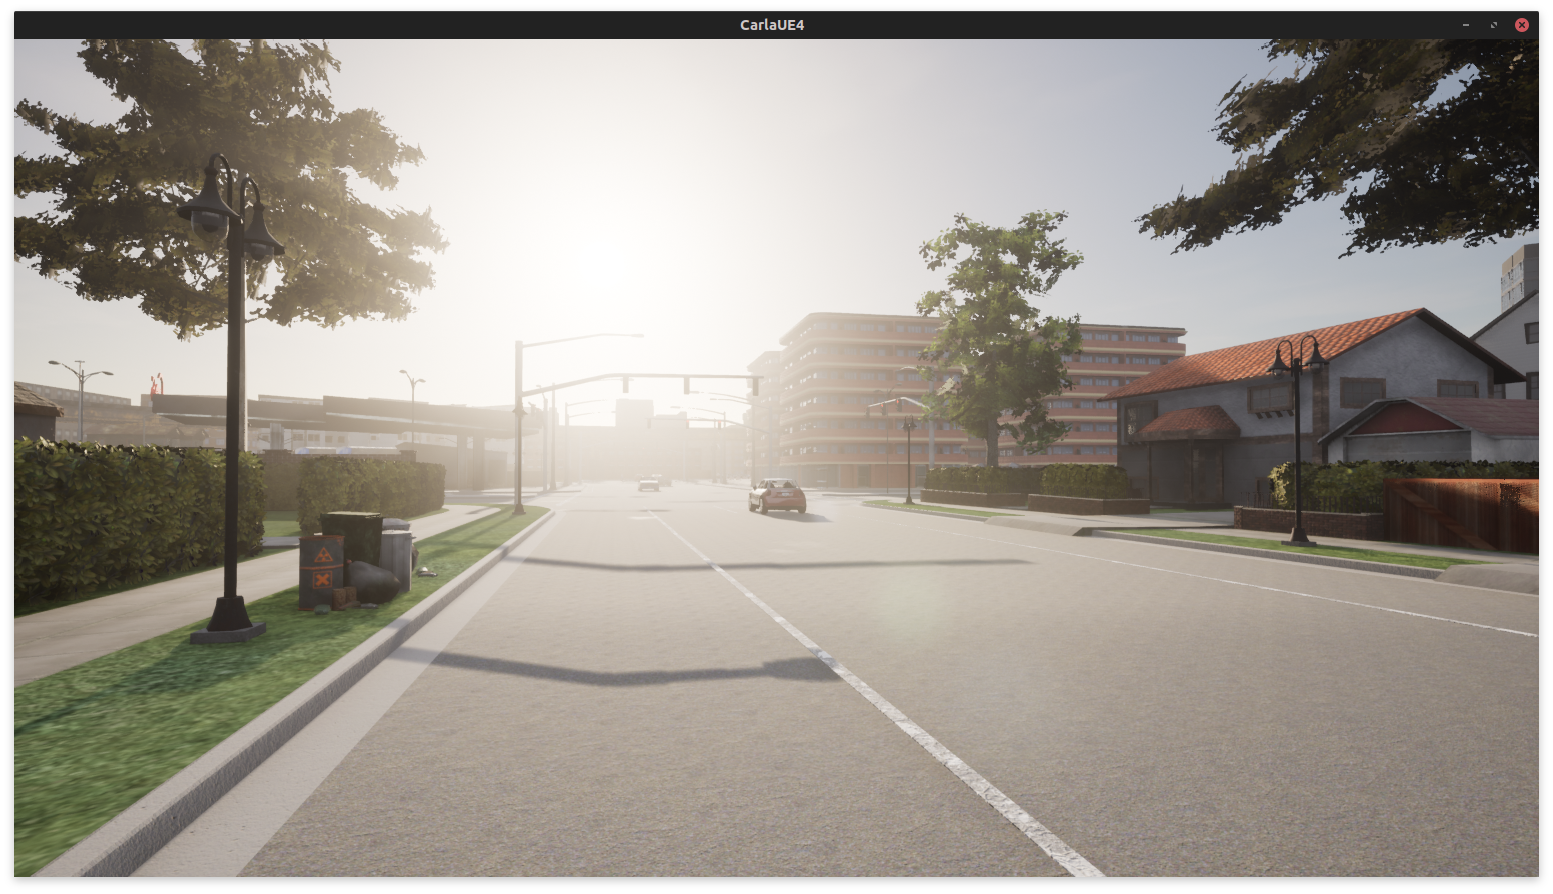
\includegraphics[width=.4\textwidth]{07_sunset.png} &
		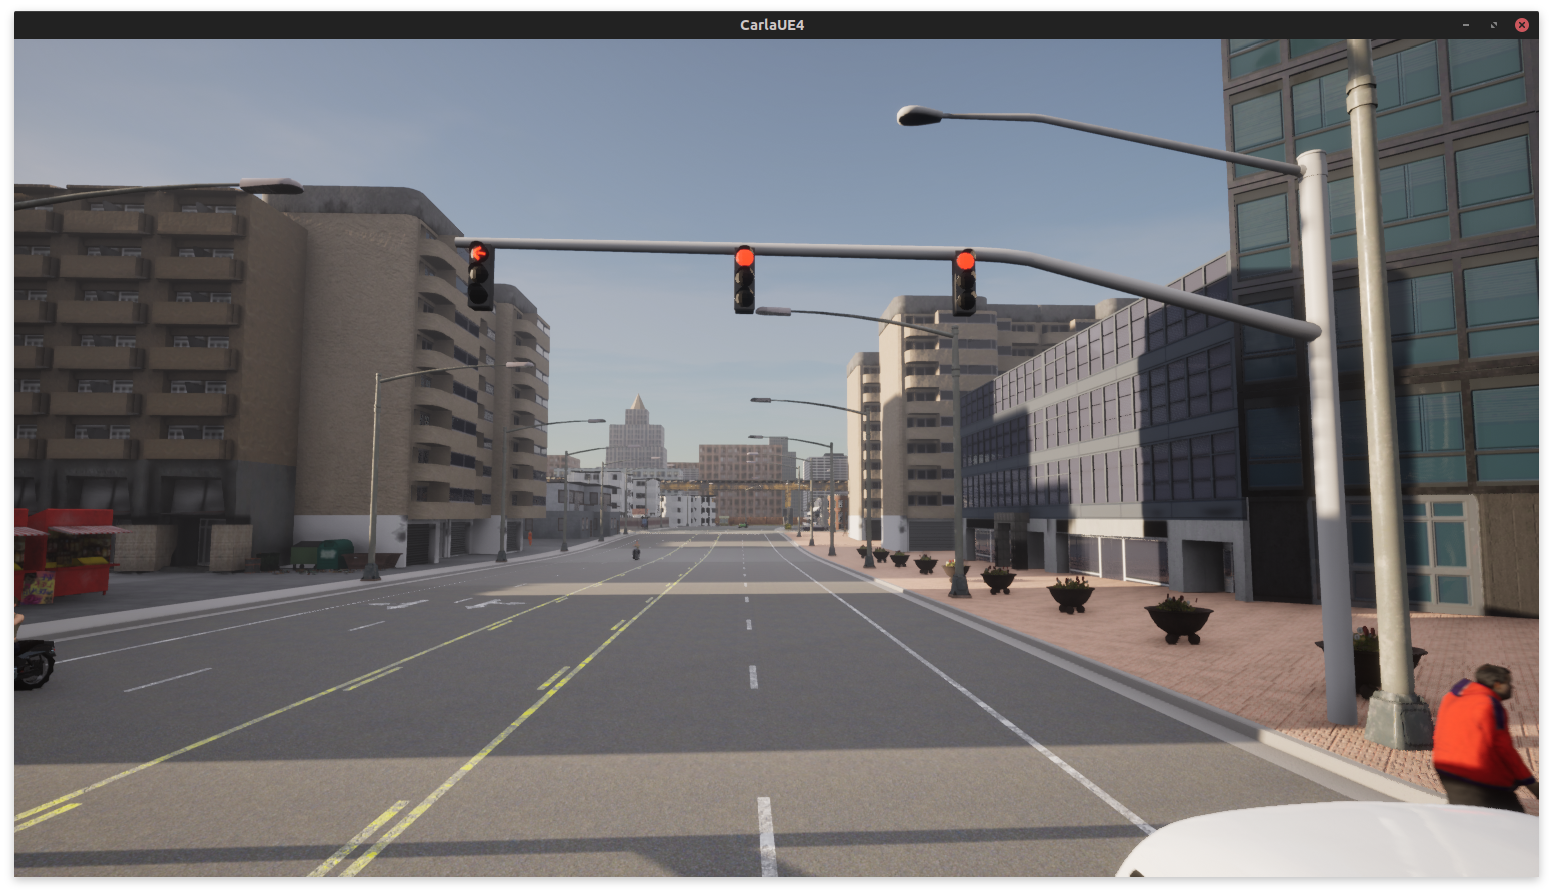
\includegraphics[width=.4\textwidth]{07_clear_sunset2.png}\\
		4 & 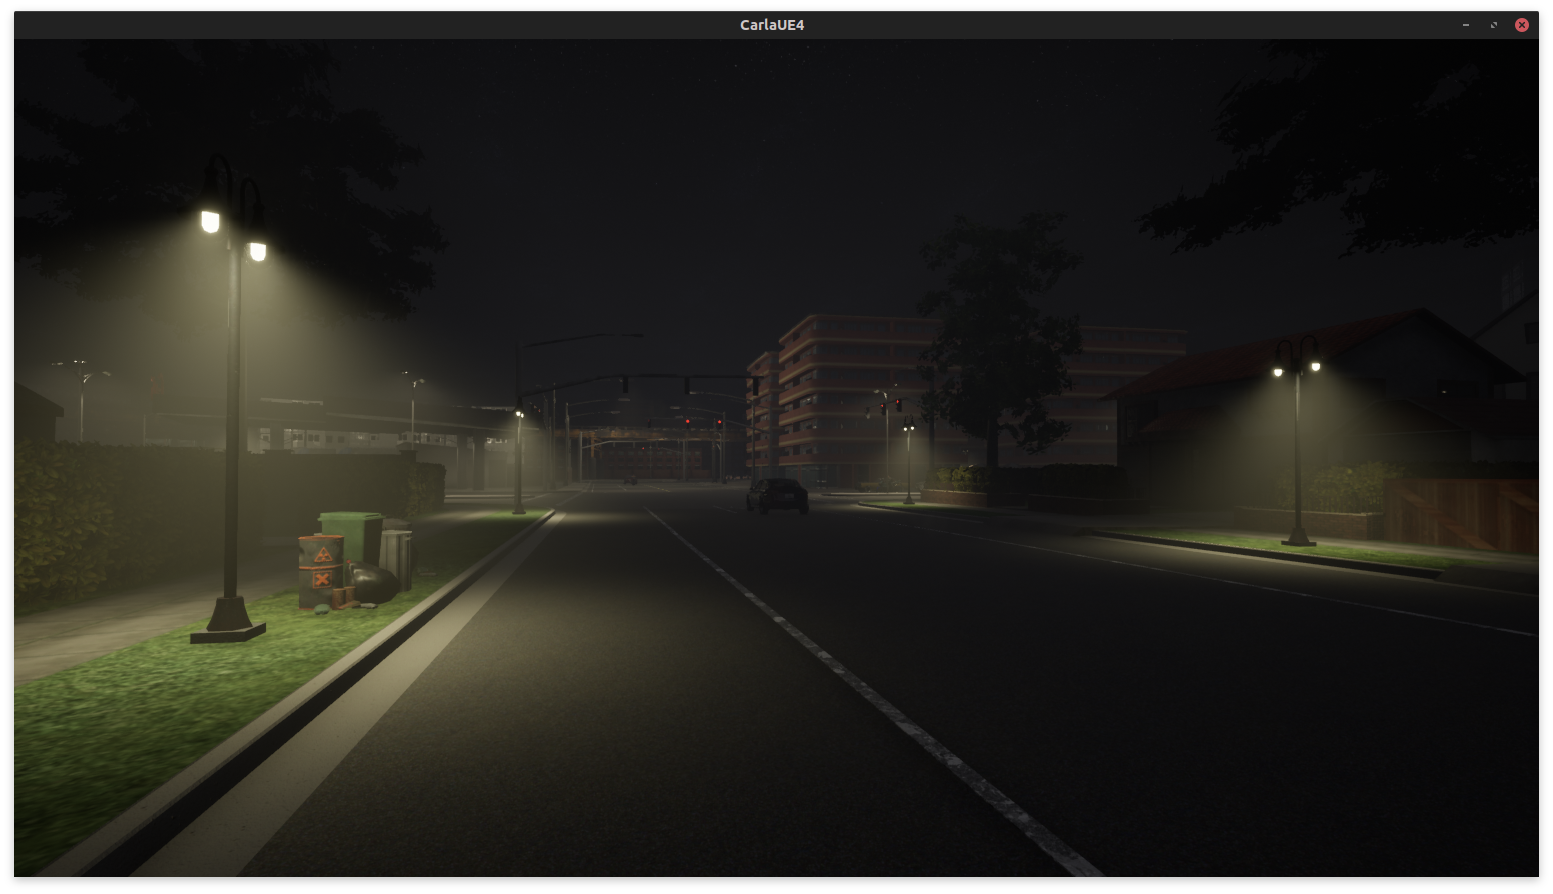
\includegraphics[width=.4\textwidth]{07_clear_night.png} &
		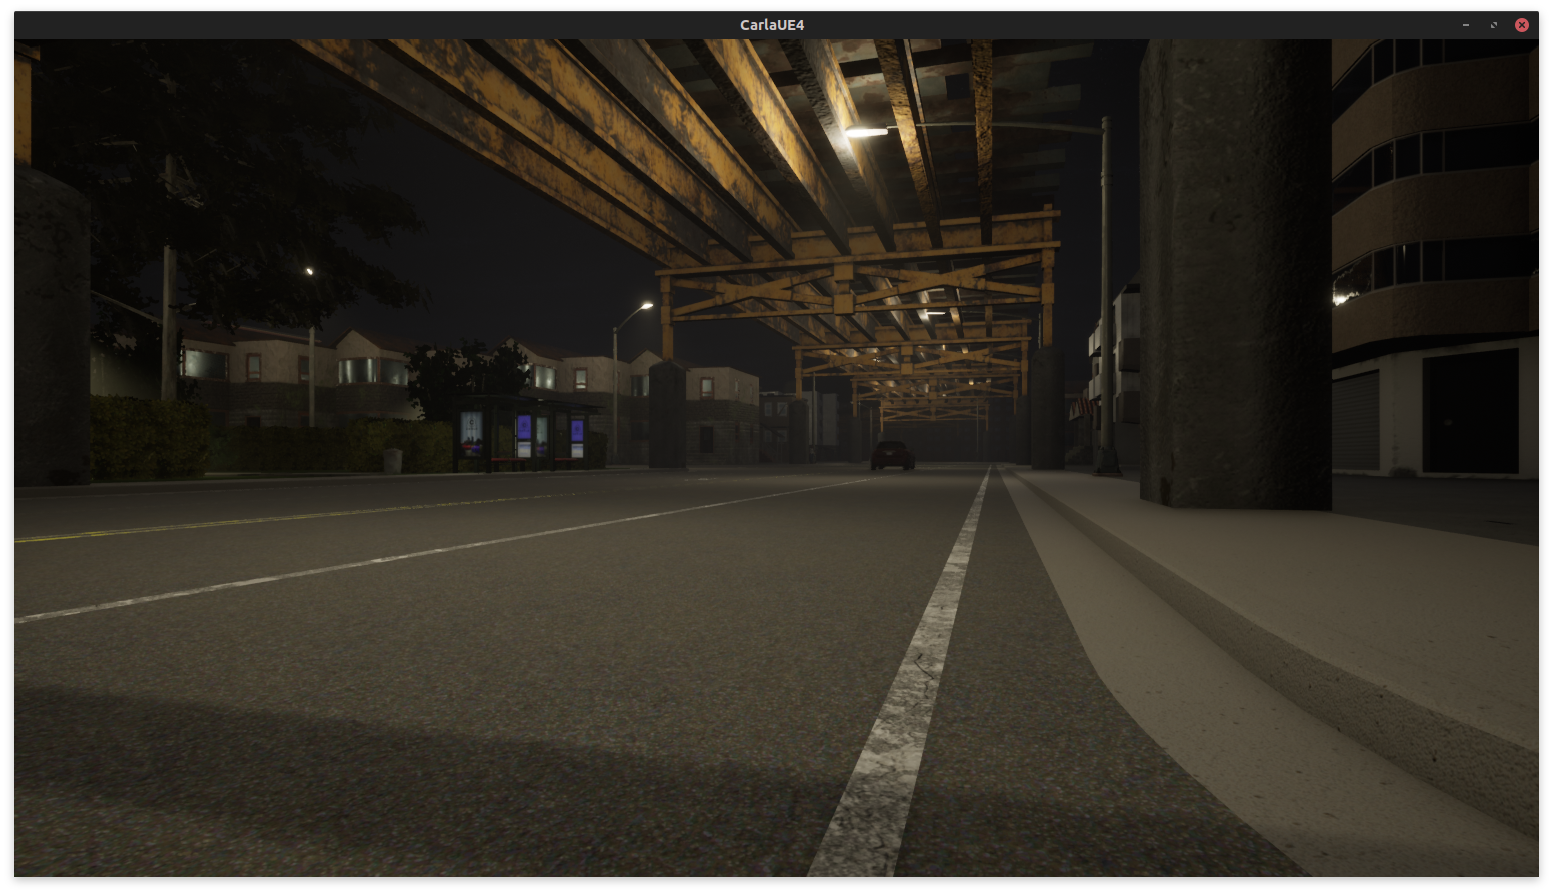
\includegraphics[width=.4\textwidth]{07_clear_night03.png}\\
		5 & 	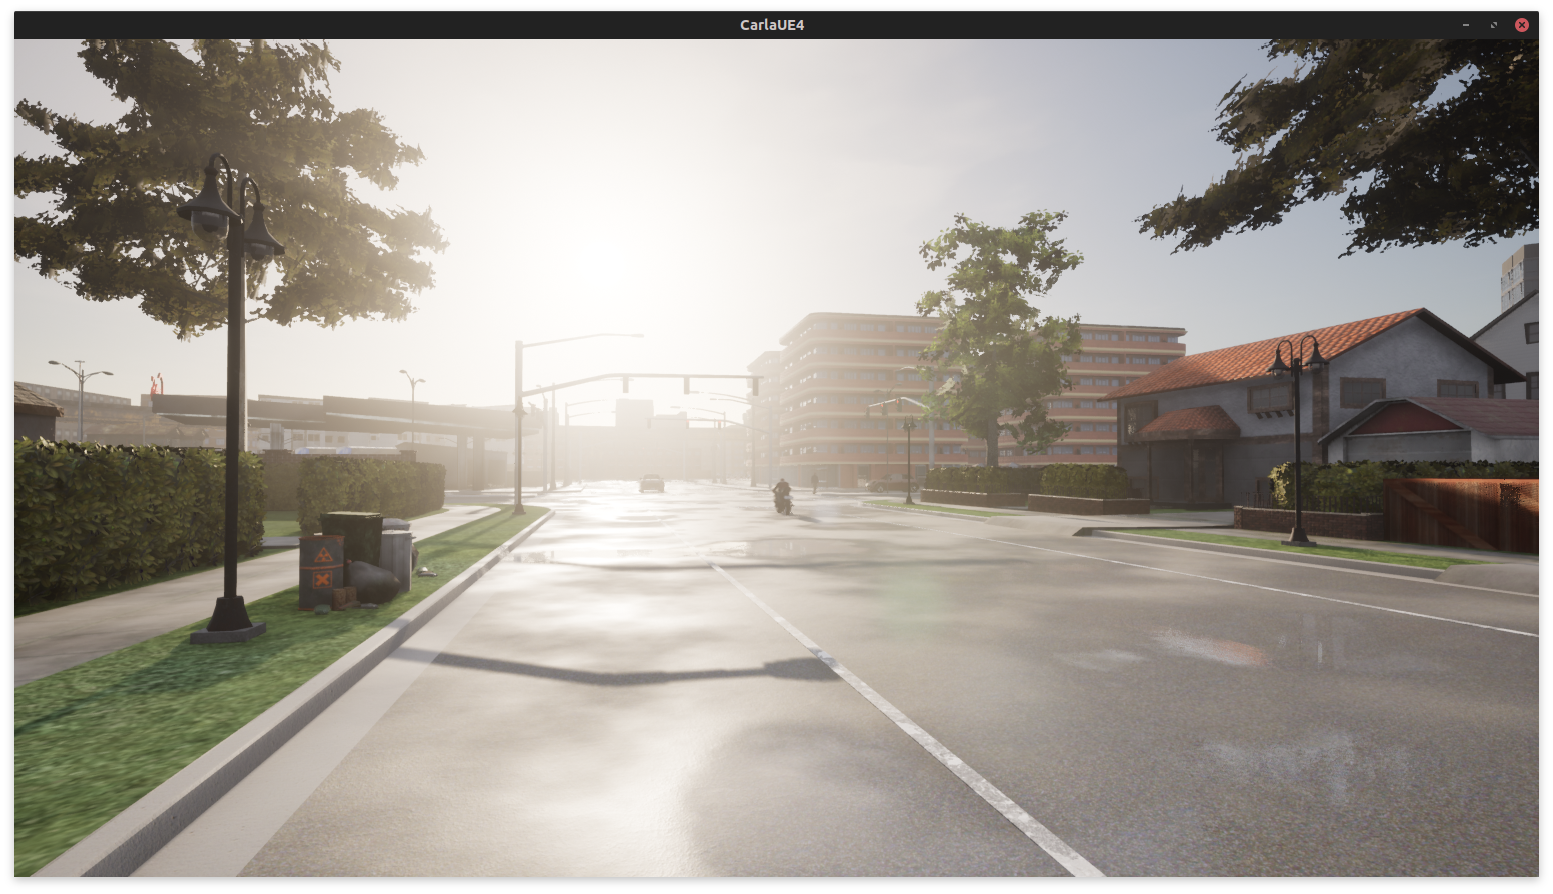
\includegraphics[width=.4\textwidth]{07_wet_sunset.png} &
		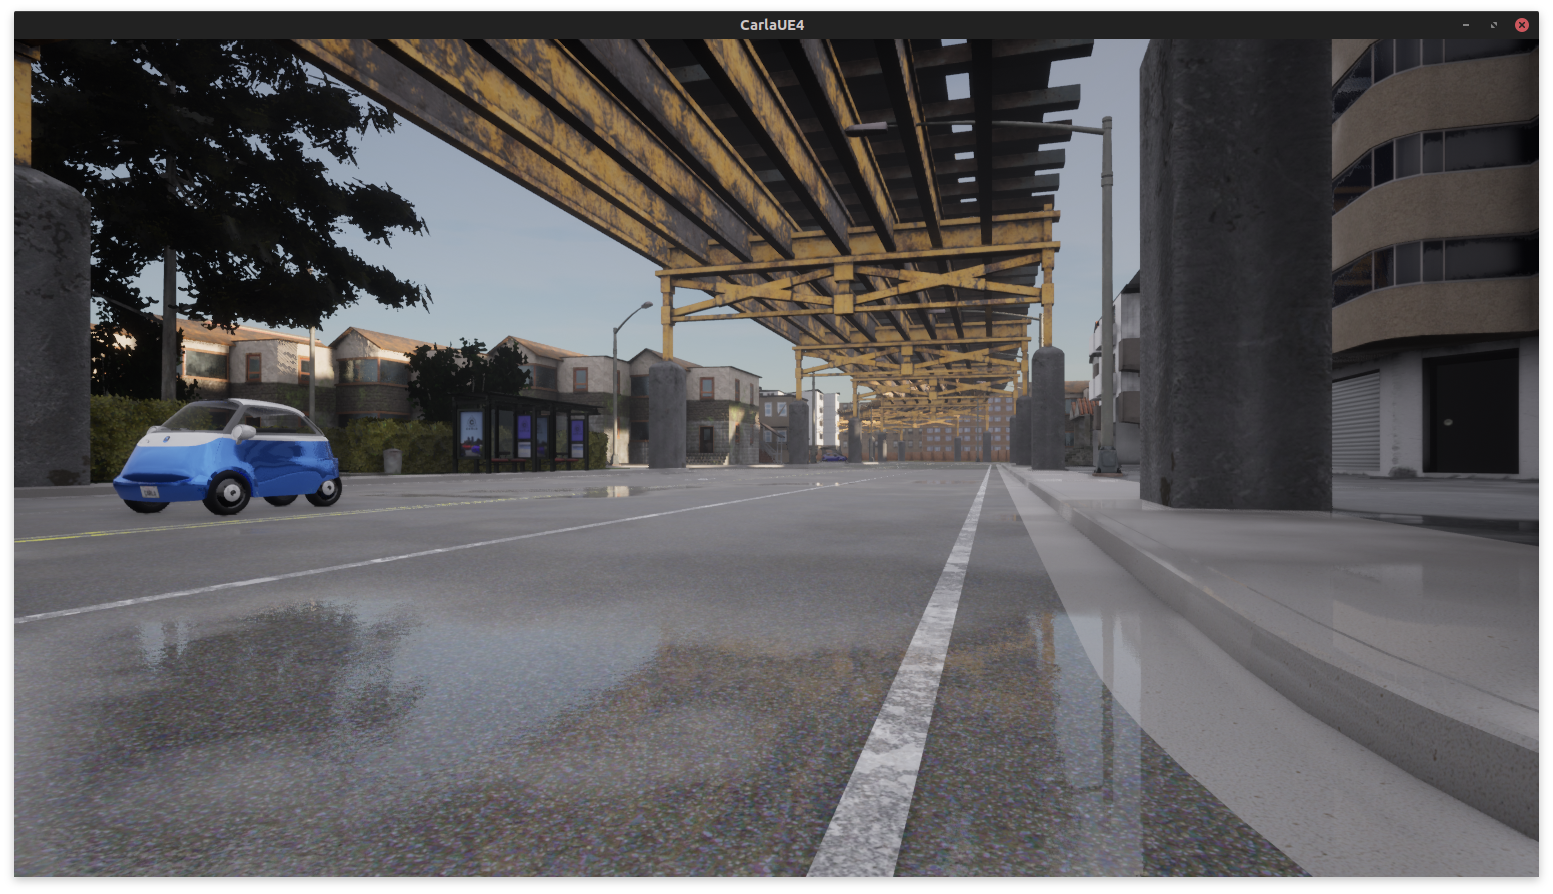
\includegraphics[width=.4\textwidth]{07_wet_sunset03.png}
		\end{tabular}
	\centering
	\caption[Witterungsverhältnisse der Simulation in verschiedenen Datensätzen]{Witterungsverhältnisse der verschiedenen Datensätze: 1 Default, 2 hard rain, 3 clear sunset, 4 clear night, 5 wet sunset}
	\label{fig:carlawetter}
\end{figure}


\newpage
\begin{figure}[!ht]
	% STEREO
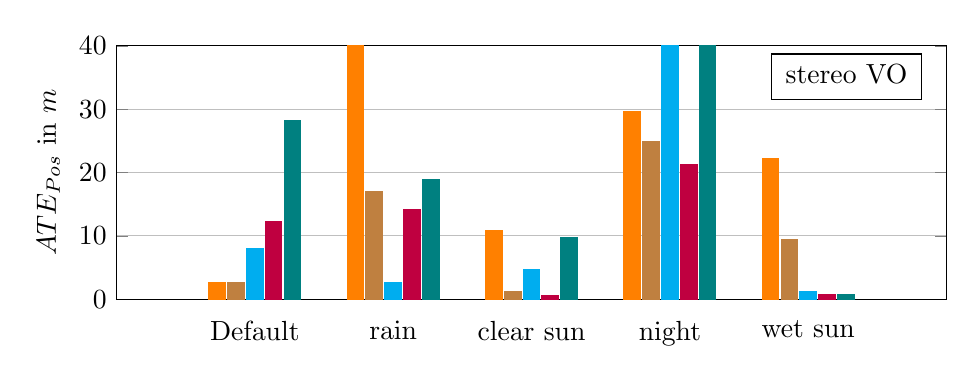
\begin{tikzpicture}
    \begin{axis}[
        width  = \textwidth,
        height = 4.8cm,
        ymax =40,
        major x tick style = transparent,
        ybar=2*\pgflinewidth,
        bar width=6pt,
        ymajorgrids = true,
        ylabel = {$ATE_{Pos}$ in $m$},
        % xlabel = {1 Default, 2 hard rain, 3 clear sunset, 4 clear night ,5 wet sunset},
        symbolic x coords={Default, rain, clear sun, night ,wet sun},
        xtick = data,
        scaled y ticks = false,
        enlarge x limits=0.25,
        ymin=0,
        legend pos=north east
    ]
    \addlegendimage{empty legend}
    \addlegendentry{stereo VO}
    \addplot[style={orange,fill=orange,mark=none}]
        coordinates {(Default, 2.70) (rain,66.61) (clear sun, 10.79) (night ,29.61) (wet sun, 22.271)};
    
    \addplot[style={brown,fill=brown,mark=none}]
        coordinates {(Default, 2.68) (rain,16.94) (clear sun, 1.16) (night , 24.96) (wet sun, 9.48)};
    
    \addplot[style={cyan,fill=cyan,mark=none}]
        coordinates {(Default, 8.07) (rain,2.663) (clear sun, 4.63) (night , 86.94) (wet sun, 1.29)};
    
    \addplot[style={purple,fill=purple,mark=none}]
        coordinates {(Default, 12.2) (rain,14.13) (clear sun, 0.569) (night ,21.32) (wet sun, .7)};
    
    \addplot[style={teal,fill=teal,mark=none}]
        coordinates {(Default, 28.2) (rain,18.87) (clear sun, 9.78) (night ,91.45) (wet sun, .7)};
    \end{axis}
  \end{tikzpicture}
	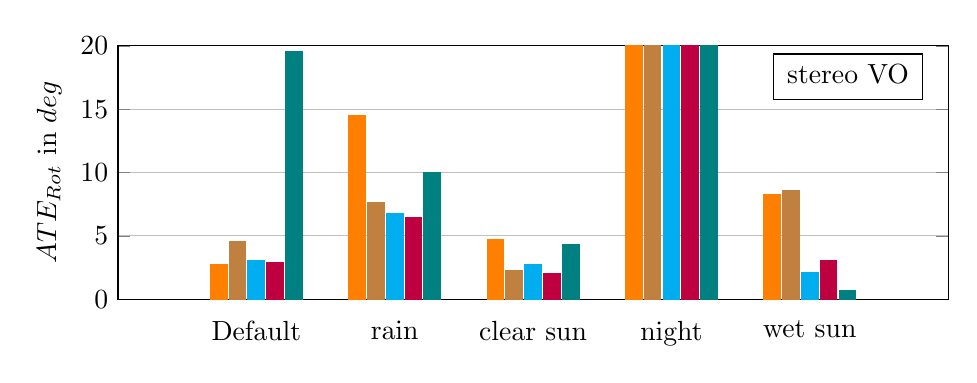
\begin{tikzpicture}
    \begin{axis}[
        width  = \textwidth,
        height = 4.8cm,
        ymax = 20,
        major x tick style = transparent,
        ybar=2*\pgflinewidth,
        bar width=6pt,
        ymajorgrids = true,
        ylabel = {$ATE_{Rot}$ in $deg$},
        % xlabel = {1 Default, 2 hard rain, 3 clear sunset, 4 clear night ,5 wet sunset},
        symbolic x coords={Default, rain, clear sun, night ,wet sun},
        xtick = data,
        scaled y ticks = false,
        enlarge x limits=0.25,
        ymin=0,
        legend pos=north east
    ]
    \addlegendimage{empty legend}
    \addlegendentry{stereo VO}
    \addplot[style={orange,fill=orange,mark=none}]
        coordinates {(Default, 2.73) (rain,14.53) (clear sun, 4.7107) (night ,44.90) (wet sun, 8.24)};
    
    \addplot[style={brown,fill=brown,mark=none}]
        coordinates {(Default, 4.52) (rain,7.65) (clear sun, 2.2452) (night ,20.45) (wet sun, 8.57)};
    
    \addplot[style={cyan,fill=cyan,mark=none}]
        coordinates {(Default, 3.05) (rain,6.74) (clear sun, 2.72) (night ,52.73) (wet sun, 2.11)};
    
    \addplot[style={purple,fill=purple,mark=none}]
        coordinates {(Default, 2.90) (rain,6.43) (clear sun, 1.99) (night , 58.59) (wet sun, 3.06)};
    
    \addplot[style={teal,fill=teal,mark=none}]
        coordinates {(Default, 19.58) (rain,9.99) (clear sun, 4.28) (night , 168.59) (wet sun, 0.672)};
    \end{axis}
  \end{tikzpicture}
	\caption[Absolute Trajectory Error (ATE) für Stereokamera]{Absolute Trajectory Error (ATE) für Stereo VO der geschätzten Translation und des geschätzten Winkels in Grad für alle 25 Testfahrten.}
	% STEREO
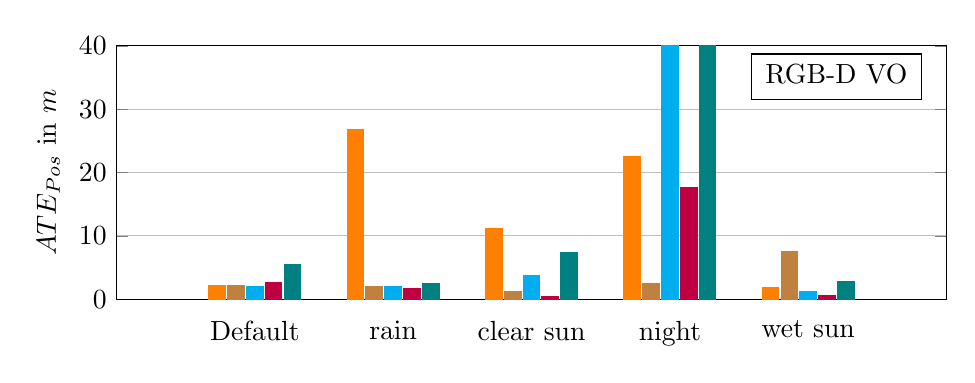
\begin{tikzpicture}
    \begin{axis}[
        width  = \textwidth,
        height = 4.8cm,
        ymax =40,
        major x tick style = transparent,
        ybar=2*\pgflinewidth,
        bar width=6pt,
        ymajorgrids = true,
        ylabel = {$ATE_{Pos}$ in $m$},
        % xlabel = {1 Default, 2 hard rain, 3 clear sunset, 4 clear night ,5 wet sunset},
        symbolic x coords={Default, rain, clear sun, night ,wet sun},
        xtick = data,
        scaled y ticks = false,
        enlarge x limits=0.25,
        ymin=0,
        legend pos=north east
    ]
    \addlegendimage{empty legend}
    \addlegendentry{RGB-D VO}

    \addplot[style={orange,fill=orange,mark=none}]
        coordinates {(Default, 2.10) (rain, 26.85) (clear sun, 11.109) (night , 22.593) (wet sun, 1.85)};
    
    \addplot[style={brown,fill=brown,mark=none}]
        coordinates {(Default, 2.16) (rain, 2.02) (clear sun, 1.28) (night , 2.518) (wet sun, 7.512)};
    
    \addplot[style={cyan,fill=cyan,mark=none}]
        coordinates {(Default, 1.94) (rain, 2.057) (clear sun, 3.768) (night , 75.997) (wet sun, 1.1535)};
    
    \addplot[style={purple,fill=purple,mark=none}]
        coordinates {(Default, 2.62) (rain, 1.648) (clear sun, 0.480) (night , 17.566) (wet sun, 0.52516)};
    
    \addplot[style={teal,fill=teal,mark=none}]
        coordinates {(Default, 5.55) (rain, 2.432) (clear sun, 7.2941) (night , 83.744) (wet sun, 2.789)};
    \end{axis}
  \end{tikzpicture}
	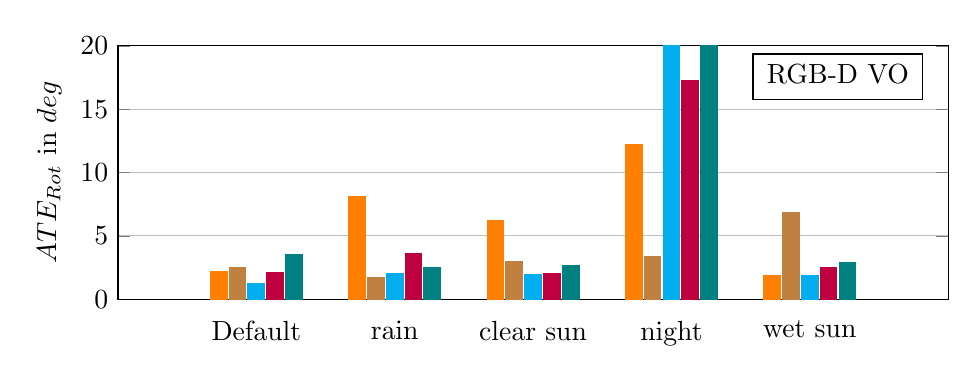
\begin{tikzpicture}
    \begin{axis}[
        width  = \textwidth,
        height = 4.8cm,
        ymax = 20,
        major x tick style = transparent,
        ybar=2*\pgflinewidth,
        bar width=6pt,
        ymajorgrids = true,
        ylabel = {$ATE_{Rot}$ in $deg$},
        % xlabel = {1 Default, 2 hard rain, 3 clear sunset, 4 clear night ,5 wet sunset},
        symbolic x coords={Default, rain, clear sun, night ,wet sun},
        xtick = data,
        scaled y ticks = false,
        enlarge x limits=0.25,
        ymin=0,
        legend pos=north east
    ]
    \addlegendimage{empty legend}
    \addlegendentry{RGB-D VO}
    \addplot[style={orange,fill=orange,mark=none}]
        coordinates {(Default, 2.21) (rain, 8.09) (clear sun, 6.195) (night ,12.18) (wet sun, 1.875)};
    
    \addplot[style={brown,fill=brown,mark=none}]
        coordinates {(Default,2.52) (rain, 1.73) (clear sun, 3.00) (night , 3.372) (wet sun, 6.825)};
    
    \addplot[style={cyan,fill=cyan,mark=none}]
        coordinates {(Default, 1.22) (rain, 2.00) (clear sun, 1.941) (night , 48.216) (wet sun, 1.838)};
    
    \addplot[style={purple,fill=purple,mark=none}]
        coordinates {(Default, 2.14) (rain, 3.60) (clear sun, 2.061) (night , 17.293) (wet sun, 2.518)};
    
    \addplot[style={teal,fill=teal,mark=none}]
        coordinates {(Default, 3.53) (rain, 2.493) (clear sun, 2.645) (night , 51.956) (wet sun, 2.893)};
    \end{axis}
  \end{tikzpicture}
	\caption[Absolute Trajectory Error (ATE) für RGB-D]{Absolute Trajectory Error (ATE) für RGB-D Visuelle Odometrie der geschätzten Translation und des geschätzten Winkels in Grad für alle 25 Testfahrten.}
\end{figure}

\begin{figure}[!ht]
	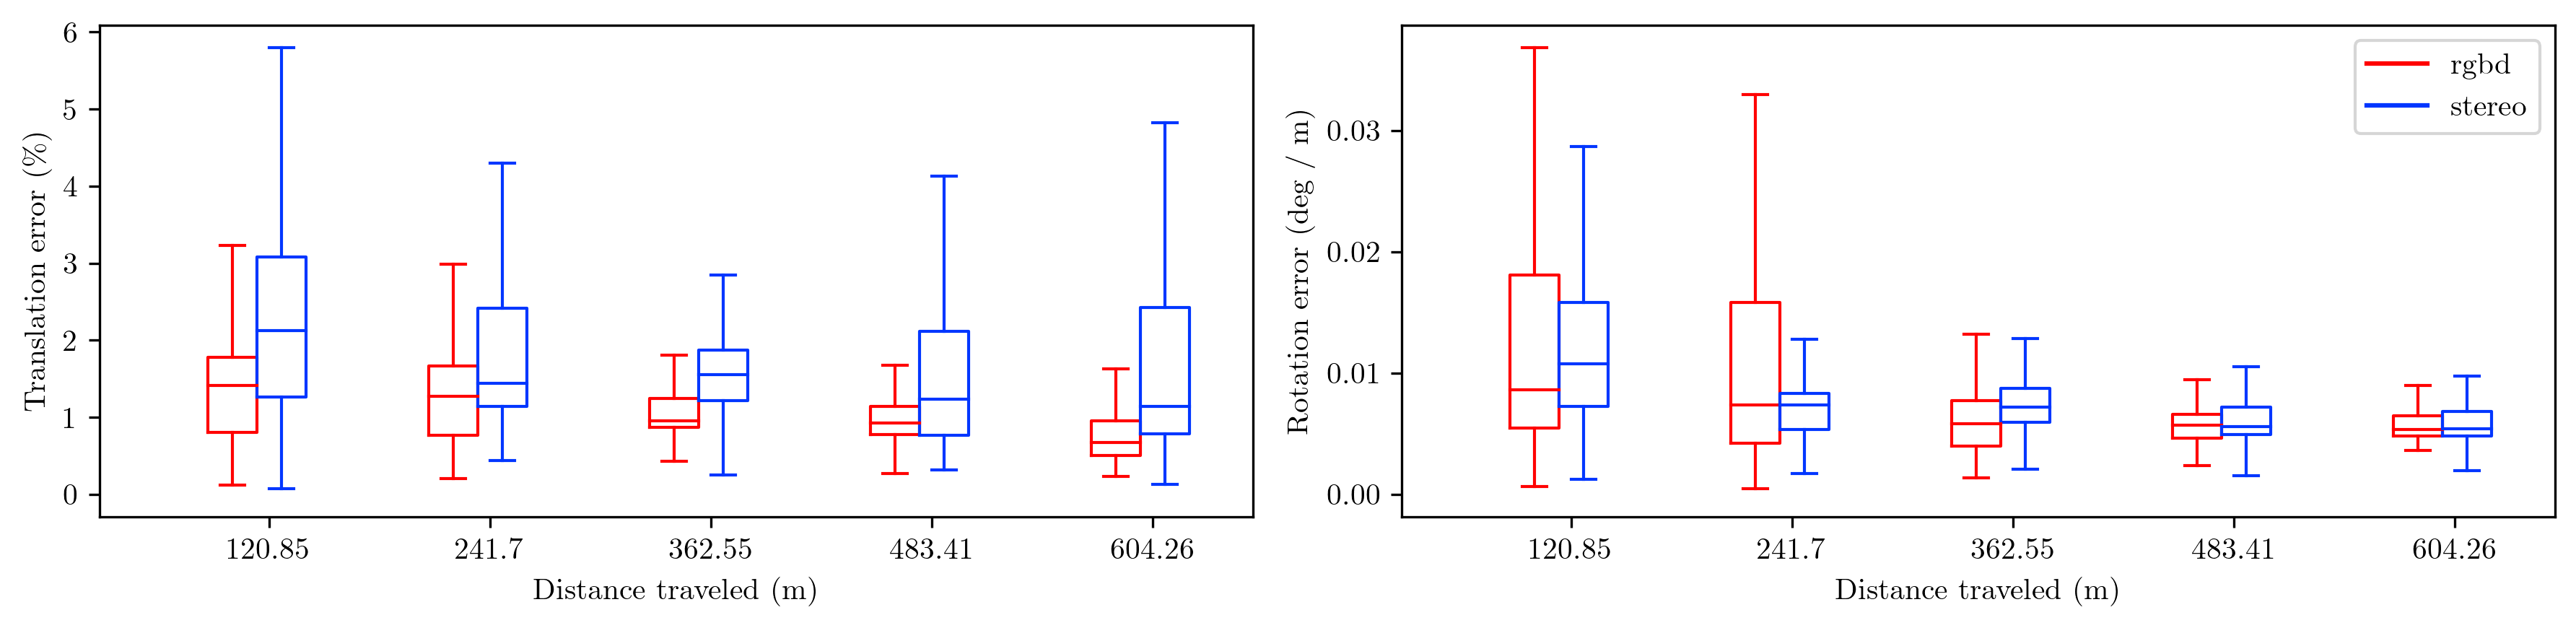
\includegraphics[width=\textwidth]{auswertung/trans_rot/default_04_trans_rot_error.png}\hfill
	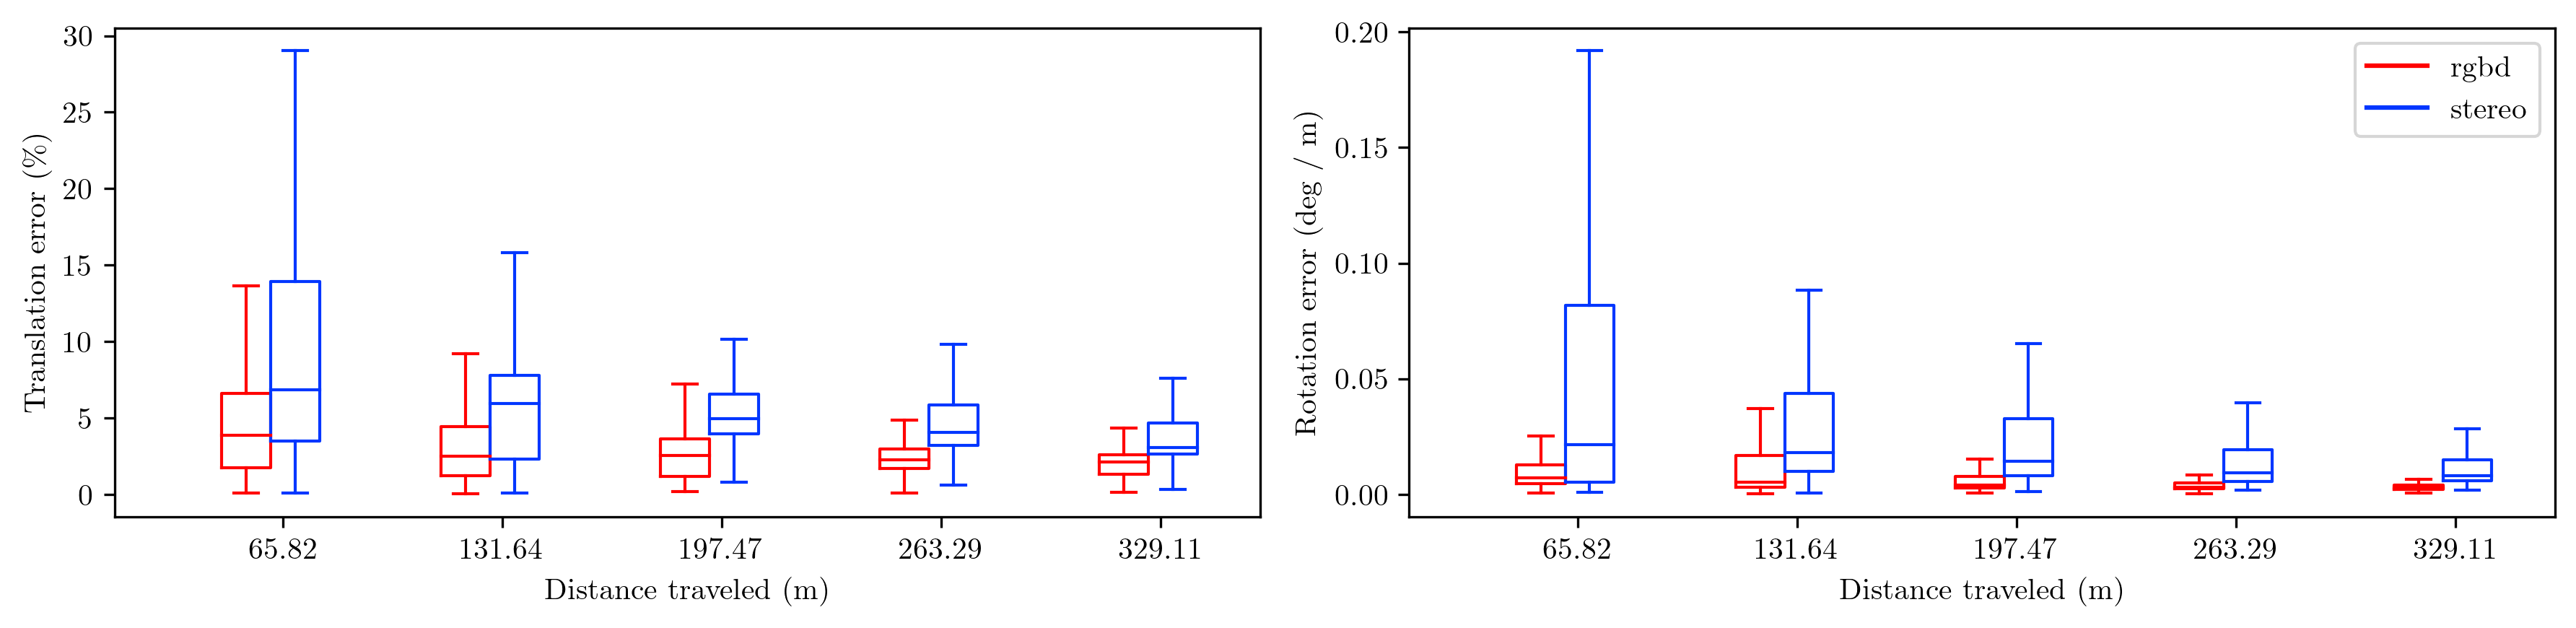
\includegraphics[width=\textwidth]{auswertung/trans_rot/hard_rain_03_trans_rot_error.png}\hfill
	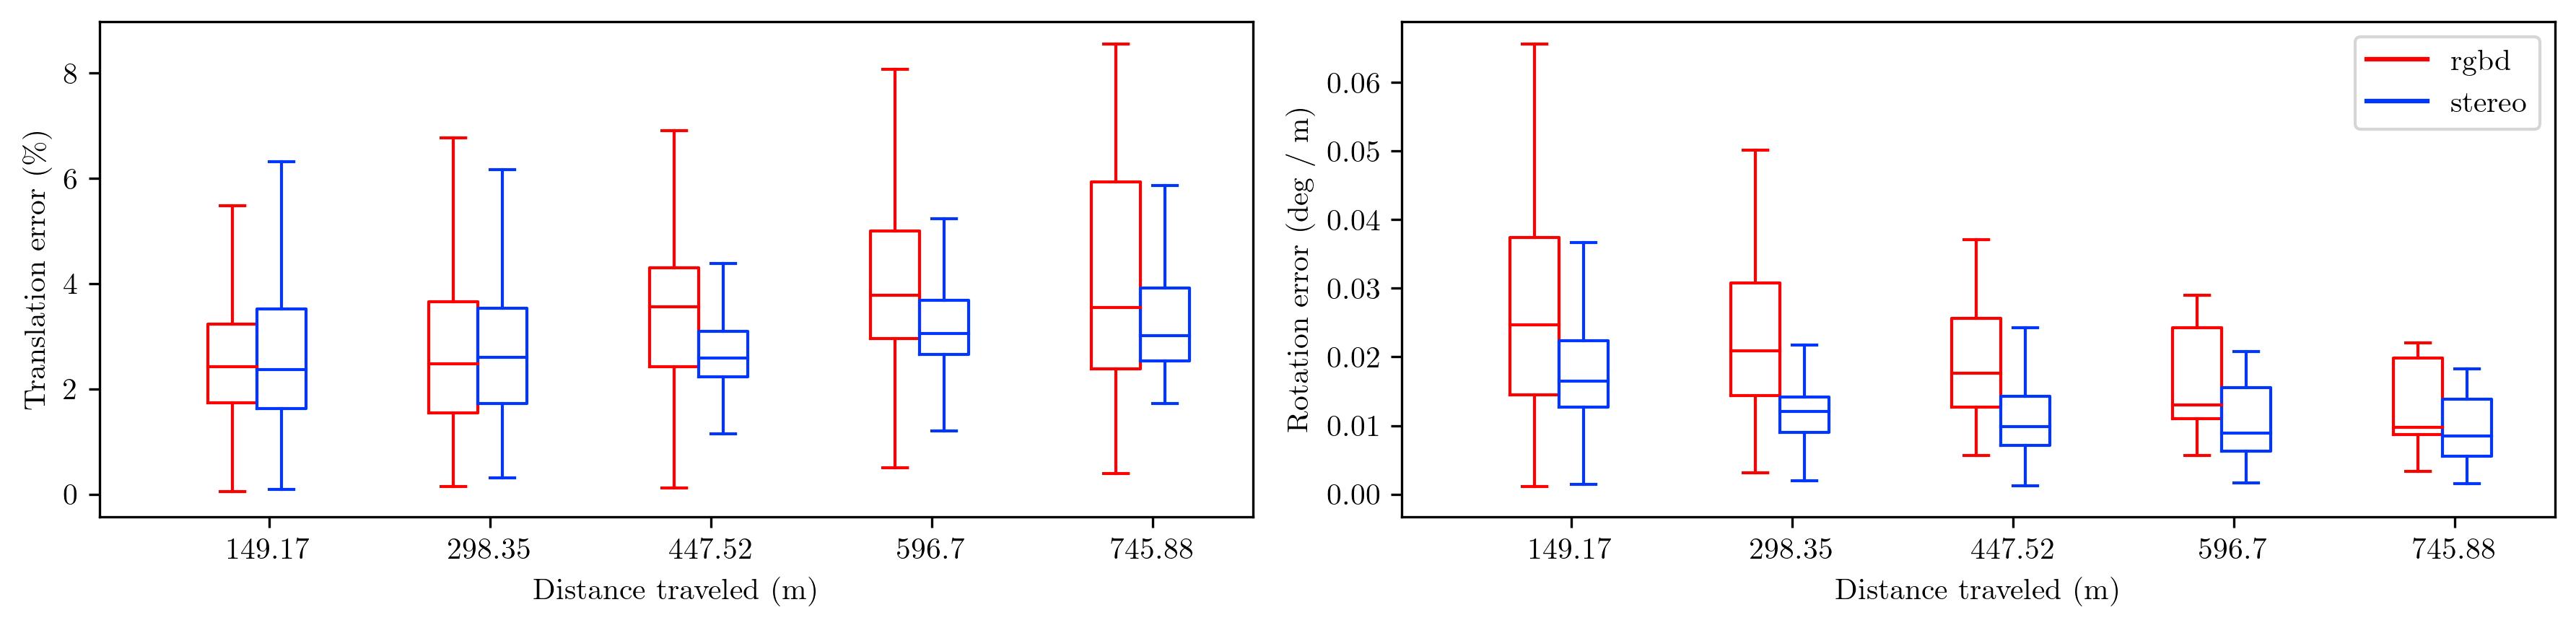
\includegraphics[width=\textwidth]{auswertung/trans_rot/sunset_01_trans_rot_error.png}
	\hfill
	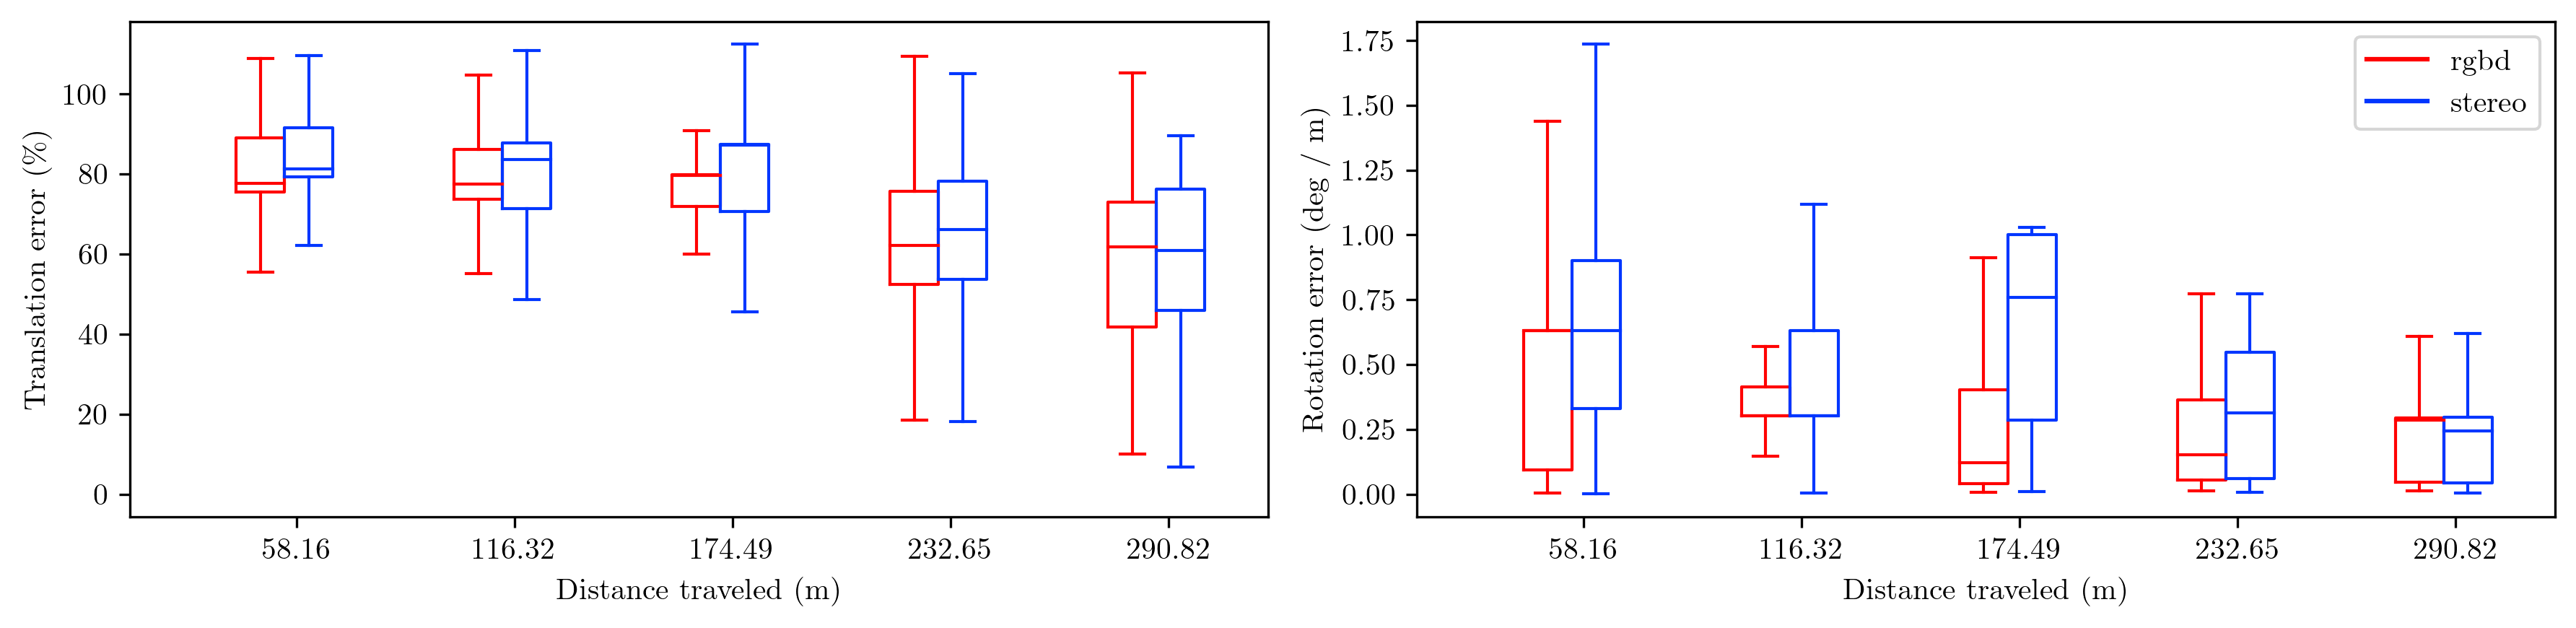
\includegraphics[width=\textwidth]{auswertung/trans_rot/clear_night_05_trans_rot_error.png}\hfill
	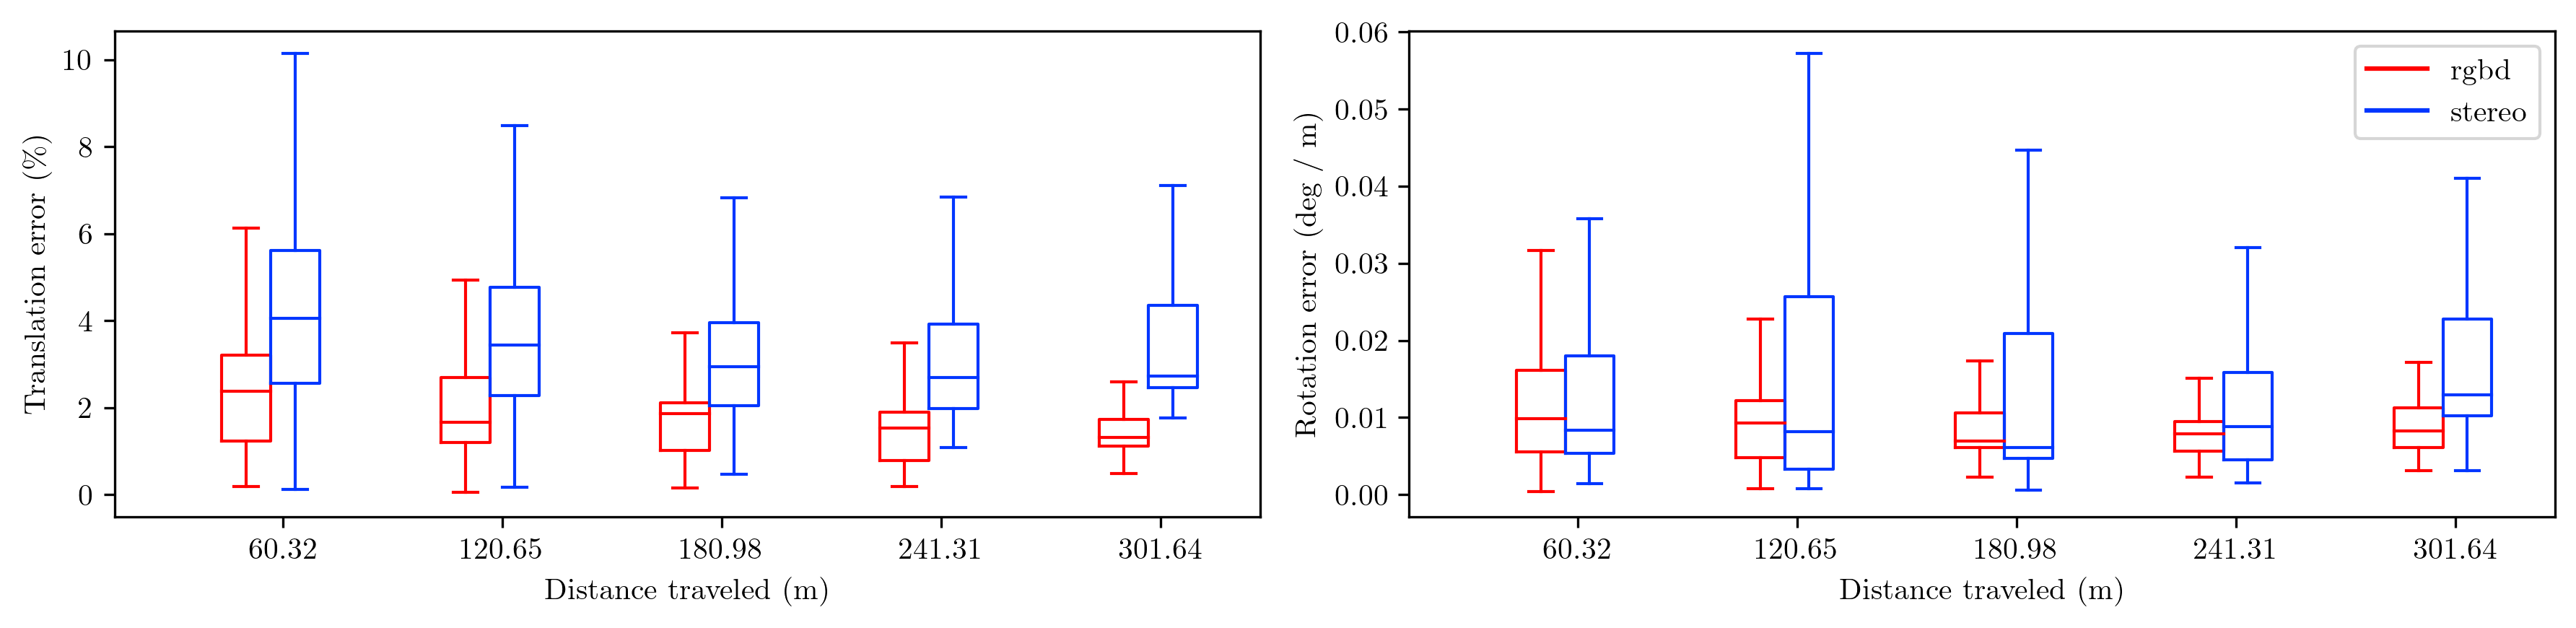
\includegraphics[width=\textwidth]{auswertung/trans_rot/wet_sunrise_01_trans_rot_error.png}\hfill
	\caption[Boxplots Absoluter Fehler von Streckenabschnitten]{Um den Trend in jedem Datensatz zu veranschaulichen wurden die Absoluten Fehler für je eine Strecke aus jedem Datensatz geplottet. Von oben nach unten: 1 Default, 2 hard rain, 3 clear sunset, 4 clear night, 5 wet sunset}
\end{figure}

\clearpage
\newpage

\begin{center}
		\begin{table}
  \centering
    \begin{tabular}{r|r|r|r|r|r}
      \toprule % <-- Toprule here
      \multicolumn{6}{c}{Median des relativen Rotations Fehlers in $deg/m$} \\
      \midrule % <-- Midrule here
      \phantom{abc} & Default & rain& clear sunset & night & wet sunset\\
      \midrule % <-- Midrule here
      (1) Stereo & 0.9452 & 4.0144 & 3.4640 & 2.9886& 2.1125\\
      \rowcolor{LightGray}
      (1) RGBD & 1.3338 & 3.1555 & 6.4847 &  0.8182& 1.5687\\
      (2) Stereo & 1.2672 & 1.0465 & 1.3600 & 3.2212& 2.1369\\
      \rowcolor{LightGray}
      (2) RGBD & 1.1546 & 1.0868 & 2.0310 &  2.5042& 1.0776\\
      (3) Stereo & 0.7136 & 1.8220 & 2.3278 & 36.9868& 0.7482\\
      \rowcolor{LightGray}
      (3) RGBD & 0.6619 &  1.6254 & 1.5180 & 38.5830& 1.1404\\
      (4) Stereo & 2.1637 &  2.4429 & 1.7825 & 53.7278& 2.4827\\
      \rowcolor{LightGray}
      (4) RGBD & 1.5119 &  3.3972 & 2.0200 & 11.9804& 2.5498\\
      (5) Stereo & 1.5989 & 4.1391 & 1.5751 & 167.3668& 1.2671\\
      \rowcolor{LightGray}
      (5) RGBD & 3.2175 & 2.1387 & 2.0686 & 34.6302&  1.8053\\	
      \bottomrule % <-- Bottomrule here
    \end{tabular}
  \caption{Median des relativer Fehlers der Rotation}
  \end{table} 	
  \begin{table}
    \centering
      \begin{tabular}{r|r|r|r|r|r}
        \toprule % <-- Toprule here
        \multicolumn{6}{c}{Median des Relativen Fehlers der Translation in $\%$} \\
        \midrule % <-- Midrule here
        \phantom{abc} & Default & rain& clear sunset & night & wet sunset\\
        \midrule % <-- Midrule here
        (1) Stereo &  2.2018 & 24.9510 & 6.8918 & 20.9637& 3.6919\\
        \rowcolor{LightGray}
        (1) RGBD & 1.6438 & 4.76527 & 9.4637 & 4.7189& 1.7361\\
        (2) Stereo & 2.4804 & 1.3636 & 0.9239 &  16.9190&  2.6304\\
        \rowcolor{LightGray}
        (2) RGBD & 1.8756 & 1.7771 & 0.9684 &  2.2069& 2.0401\\
        (3) Stereo & 1.4768 & 5.1681 & 4.1606 & 61.4019& 0.8780\\
        \rowcolor{LightGray}
        (3) RGBD & 1.2665 & 1.6829 & 3.2752 & 63.2587& 0.9144\\
        (4) Stereo & 2.6105 &  3.8872 & 0.0473 & 16.1462& 0.1121\\
        \rowcolor{LightGray}
        (4) RGBD & 2.1176 & 1.3754 &  0.1263 & 9.0187& 0.0566\\
        (5) Stereo &  17.3331 &  6.1409 & 3.4013 & 55.5880&0.9190\\
        \rowcolor{LightGray}
        (5) RGBD & 5.3631 &  1.4550 & 4.1606 & 48.8802& 2.2763\\	
        \bottomrule % <-- Bottomrule here
      \end{tabular}
    \caption{Median des Relativen Fehlers der Translation}
  \end{table} 		
\end{center}
\newpage
\begin{center}
		
  \begin{table}
    \centering
      \begin{tabular}{r|r|r|r|r|r}
        \toprule % <-- Toprule here
        \multicolumn{6}{c}{RMSE der Rotation in $deg/m$} \\
        \midrule % <-- Midrule here
        \phantom{abc} & Default & rain& clear sunset & night & wet sunset\\
        \midrule % <-- Midrule here
        (1) Stereo & 2.7334 & 14.5396 & 4.7107 & 29.6143& 8.2440\\
        \rowcolor{LightGray}
        (1) RGBD & 2.2146 & 8.0921 & 6.1959 & 12.1838& 1.8756\\
        (2) Stereo & 4.5297 & 7.6523 & 2.2452 & 20.4506& 8.5746\\
        \rowcolor{LightGray}
        (2) RGBD & 2.5232 & 1.7378 & 3.0055 & 3.3728& 6.8255\\
        (3) Stereo & 3.0501 & 6.7407 & 2.7294 & 52.7385& 2.1195\\
        \rowcolor{LightGray}
        (3) RGBD & 1.2257 & 2.0066 &  1.9411 & 48.2168& 1.8383\\
        (4) Stereo & 2.9097 & 6.4370 & 1.9908 & 58.5951& 3.0643\\
        \rowcolor{LightGray}
        (4) RGBD & 2.1487 & 3.6022 & 2.0612 & 17.2936&2.5188\\
        (5) Stereo & 19.5840 &  9.9986 & 4.2870 & 168.5980& 2.0029\\
        \rowcolor{LightGray}
        (5) RGBD & 3.2175 & 2.4937 & 2.6455 & 51.9567& 2.8930\\	
        \bottomrule % <-- Bottomrule here
      \end{tabular}
    \caption{RMSE der Rotation}
  \end{table} 	
  \begin{table}
    \centering
      \begin{tabular}{r|r|r|r|r|r}
        \toprule % <-- Toprule here
        \multicolumn{6}{c}{RMSE der Translation in $\%$} \\
        \midrule % <-- Midrule here
        \phantom{abc} & Default & rain& clear sunset & night & wet sunset\\
        \midrule % <-- Midrule here
        (1) Stereo & 2.7093 & 66.6148 & 10.7996 & 44.9045&  22.2712\\
        \rowcolor{LightGray}
        (1) RGBD & 2.1084 & 26.8571 &11.1097 & 22.5937& 1.8512\\
        (2) Stereo & 2.6822 & 16.9418 & 1.1682 & 24.9654& 9.4863\\
        \rowcolor{LightGray}
        (2) RGBD &  2.1633 & 2.0260 & 1.2843 & 2.5186& 7.5126\\
        (3) Stereo & 8.0751 & 26.6375 & 4.6390 & 86.9499& 1.2902\\
        \rowcolor{LightGray}
        (3) RGBD & 1.9449 & 2.0570 & 3.76853 & 75.9970& 1.1535\\
  
        (4) Stereo & 12.2844 & 14.1325 &  0.5691 & 21.3222& 0.6728\\
        \rowcolor{LightGray}
        (4) RGBD & 2.6251 & 1.6480 & 0.4805 & 17.5666& 0.5251\\
        (5) Stereo & 28.2357 & 18.8744 & 9.7872 & 91.4595& 1.2994\\
        \rowcolor{LightGray}
        (5) RGBD & 5.5522 & 2.4321 & 7.2941 & 83.7440&  2.7893\\	
        \bottomrule % <-- Bottomrule here
      \end{tabular}
    \caption{RMSE der Translation}
  \end{table} 		
\end{center}

\newpage
\clearpage
\newpage

\section{Diskussion}
Die RMSE Tabellen zeigen die Standardabweichung für die Schätzfehler der beiden Visuellen Odometrie Systeme RGB-D und Stereo Kamera. Die Standardabweichung zeigt wie sehr die Schätzungen um den Mittelwert Streuen. Die Median Tabellen zeigen die gemittelten Fehlerwerte mit geringeren Bewertung für Ausrei{\ss}er.
\newline 

Es ist sofort ersichtlich, dass die implementierte visuelle Odometrie unbrauchbare Ergebnisse für Nachtfahrten liefert. Es wäre interessant zu sehen, in wie fern sich die Ergebnisse für Fahrten mit Frontscheinwerfern ändern. Da Stra{\ss}en, insbesondere Asphalt, eine Textur arme Oberflächentextur bieten, würden die Kamerabilder aus der RGB Kamera vermutlich dennoch nicht genug Merkmale beinhalten.   
\newline 

Der Schätzfehler mit Stereokamera streut stärker als für den RGB-D au{\ss}er für 'Clear Sunset' wo ein sehr niedriger Sonnenstand vorherrscht.  
\newline

In der Auswertung des Gesamtstreckenfehlers zeigt sich, dass der RGB-D Kameraaufbau insgesamt kleinere Schätzfehler hat. Mit weniger Streuung ist es auch das Robustere System.    
\newline

Keines der Systeme zeigte Auffälligkeiten bei Ein- und Ausfahrten des in der Karte integrierten Tunnel. Bei hohen Geschwindigkeiten $(> 80 km\/h)$ kam es vermehrt zum Verlust der Schätzung, vor allem auf Streckenabschnitten mit wenigen markanten Umgebungsmerkmalen.  
\newline

Insgesamt konnte gezeigt werden, dass eine Lokalisierung des Fahrzeugs alleine durch Visuelle Odmometrie erfolgreich durchgeführt werden konnte. Beide Systeme liefern i.d.R. bei Tageslicht weniger als 10 Grad Winkelfehler. Die Visuelle Odometrie mit RGB-D Kamera schafft in 17 von 25 Teststrecken einen einen Absoluten Streckenfehler von weniger als 5 Metern. 

\section{Ausblick}
Das System kann als Front-End für einen SLAM Algorithmus verwendet werden. Bei einigen Testfahrten hat sich die Odometrie von einer gro{\ss}en Fehlschätzung vor allem nie 'erholt', vor allem dann, wenn der Fehler zu Beginn auftrat. Durch SLAM könnten solche Verläufe stabilisiert werden und das gesamte Verfahren würde Robuster werden. 
\newline

Eine weitere, naheliegende Möglichkeit wäre eine Sensorfusion mit einer IMU. Sogenannte Visual Inertial Odometry zeigt in aktuellen Forschungsergebnissen mehrere Paper gute Ergebnisse für eine Fehlerkorrektur und damit eine Reduktion der Drift.